\documentclass[a4paper,12pt]{report}
\usepackage[utf8]{inputenc}
\usepackage[T1]{fontenc}
\usepackage[english]{babel}
\usepackage{lmodern}
\usepackage{enumitem}

% References Packages
\usepackage{xr-hyper}
% hyperref for interactive PDF index
\usepackage[bookmarks, colorlinks, breaklinks]{hyperref}
\hypersetup{linkcolor=black, citecolor=black, filecolor=black, urlcolor=black}

% Package required to use special symbols
\usepackage{amsmath, amssymb}

% Package for tables
\usepackage{tabu}
\usepackage{tabularx}
\usepackage{ltablex}
\usepackage{longtable}
\usepackage{float} % To allow the use of H modifier in long tables
\usepackage{multirow}

% Package required to use figures
\usepackage{graphicx}
\usepackage{wrapfig}

% Package used to insert figures at the specified position
\usepackage{float} 

% To have a new line after a \paragraph
\newcommand{\customParagraph}[1]{\paragraph{#1}\mbox{}\\}

% Paragraph indent
\setlength{\parindent}{0pt}

% Special chars
\usepackage{textcomp}

\makeatletter
\usepackage{color}
\definecolor{lightgray}{rgb}{0.95, 0.95, 0.95}
\definecolor{darkgray}{rgb}{0.4, 0.4, 0.4}
%\definecolor{purple}{rgb}{0.65, 0.12, 0.82}
\definecolor{editorGray}{rgb}{0.95, 0.95, 0.95}
\definecolor{editorOcher}{rgb}{1, 0.5, 0} % #FF7F00 -> rgb(239, 169, 0)
\definecolor{editorGreen}{rgb}{0, 0.5, 0} % #007C00 -> rgb(0, 124, 0)
\definecolor{orange}{rgb}{1,0.45,0.13}		
\definecolor{olive}{rgb}{0.17,0.59,0.20}
\definecolor{brown}{rgb}{0.69,0.31,0.31}
\definecolor{purple}{rgb}{0.38,0.18,0.81}
\definecolor{lightblue}{rgb}{0.1,0.57,0.7}
\definecolor{lightred}{rgb}{1,0.4,0.5}
\usepackage{upquote}
\usepackage{listings}
% CSS
\lstdefinelanguage{CSS}{
  keywords={color,background-image:,margin,padding,font,weight,display,position,top,left,right,bottom,list,style,border,size,white,space,min,width, transition:, transform:, transition-property, transition-duration, transition-timing-function},	
  sensitive=true,
  morecomment=[l]{//},
  morecomment=[s]{/*}{*/},
  morestring=[b]',
  morestring=[b]",
  alsoletter={:},
  alsodigit={-}
}

% JavaScript
\lstdefinelanguage{JavaScript}{
  morekeywords={typeof, new, true, false, catch, function, return, null, catch, switch, var, if, in, while, do, else, case, break},
  morecomment=[s]{/*}{*/},
  morecomment=[l]//,
  morestring=[b]",
  morestring=[b]'
}

\lstdefinelanguage{HTML5}{
  language=html,
  sensitive=true,	
  alsoletter={<>=-},	
  morecomment=[s]{<!-}{-->},
  tag=[s],
  otherkeywords={
  % General
  >,
  % Standard tags
	<!DOCTYPE,
  </html, <html, <head, <title, </title, <style, </style, <link, </head, <meta, />,
	% body
	</body, <body,
	% Divs
	</div, <div, </div>, 
	% Paragraphs
	</p, <p, </p>,
	% scripts
	</script, <script,
  % More tags...
  <canvas, /canvas>, <svg, <rect, <animateTransform, </rect>, </svg>, <video, <source, <iframe, </iframe>, </video>, <image, </image>, <header, </header, <article, </article
  },
  ndkeywords={
  % General
  =,
  % HTML attributes
  charset=, src=, id=, width=, height=, style=, type=, rel=, href=,
  % SVG attributes
  fill=, attributeName=, begin=, dur=, from=, to=, poster=, controls=, x=, y=, repeatCount=, xlink:href=,
  % properties
  margin:, padding:, background-image:, border:, top:, left:, position:, width:, height:, margin-top:, margin-bottom:, font-size:, line-height:,
	% CSS3 properties
  transform:, -moz-transform:, -webkit-transform:,
  animation:, -webkit-animation:,
  transition:,  transition-duration:, transition-property:, transition-timing-function:,
  }
}

\lstdefinestyle{htmlcssjs} {%
  % General design
%  backgroundcolor=\color{editorGray},
  basicstyle={\footnotesize\ttfamily},   
  frame=b,
  % line-numbers
  xleftmargin={0.75cm},
  numbers=left,
  stepnumber=1,
  firstnumber=1,
  numberfirstline=true,	
  % Code design
  identifierstyle=\color{black},
  keywordstyle=\color{blue}\bfseries,
  ndkeywordstyle=\color{editorGreen}\bfseries,
  stringstyle=\color{editorOcher}\ttfamily,
  commentstyle=\color{brown}\ttfamily,
  % Code
  language=HTML5,
  alsolanguage=JavaScript,
  alsodigit={.:;},	
  tabsize=2,
  showtabs=false,
  showspaces=false,
  showstringspaces=false,
  extendedchars=true,
  breaklines=true,
  % German umlauts
  literate=%
  {Ö}{{\"O}}1
  {Ä}{{\"A}}1
  {Ü}{{\"U}}1
  {ß}{{\ss}}1
  {ü}{{\"u}}1
  {ä}{{\"a}}1
  {ö}{{\"o}}1
}
%
\lstdefinestyle{py} {%
language=python,
literate=%
*{0}{{{\color{lightred}0}}}1
{1}{{{\color{lightred}1}}}1
{2}{{{\color{lightred}2}}}1
{3}{{{\color{lightred}3}}}1
{4}{{{\color{lightred}4}}}1
{5}{{{\color{lightred}5}}}1
{6}{{{\color{lightred}6}}}1
{7}{{{\color{lightred}7}}}1
{8}{{{\color{lightred}8}}}1
{9}{{{\color{lightred}9}}}1,
basicstyle=\footnotesize\ttfamily, % Standardschrift
numbers=left,               % Ort der Zeilennummern
%numberstyle=\tiny,          % Stil der Zeilennummern
%stepnumber=2,               % Abstand zwischen den Zeilennummern
numbersep=5pt,              % Abstand der Nummern zum Text
tabsize=4,                  % Groesse von Tabs
extendedchars=true,         %
breaklines=true,            % Zeilen werden Umgebrochen
keywordstyle=\color{blue}\bfseries,
frame=b,
commentstyle=\color{brown}\itshape,
stringstyle=\color{editorOcher}\ttfamily, % Farbe der String
showspaces=false,           % Leerzeichen anzeigen ?
showtabs=false,             % Tabs anzeigen ?
xleftmargin=17pt,
framexleftmargin=17pt,
framexrightmargin=5pt,
framexbottommargin=4pt,
%backgroundcolor=\color{lightgray},
showstringspaces=false,      % Leerzeichen in Strings anzeigen ?
}%
%
\makeatother

%% ----------------------------------------------------
%% --------------------- DOCUMENT ---------------------
%% ----------------------------------------------------

\begin{document}

% Title page
\begin{titlepage}
\centering
	\begin{center}{
		\begin{figure}[h]
		\large
		\centering
		{
\includegraphics[width=.70\linewidth]{img/logo_poli}}
        \end{figure}
    	}
	\end{center}
	\vspace{1 cm}
	{\Large {\textbf{\LARGE MOQA} \\
		Design and Implementation of a Mobile Application \\ Prof. Luciano Baresi \\ 2019/2020} \par}
	\vspace{1.5cm}
	{\LARGE \textbf{Design and Technology} \par}
	{\Large\itshape Mathyas Giudici\par}
	\vfill
	% Bottom of the page
	{\large Document version: 1.0\par}
	{\large \today \par}
\end{titlepage}

{
\pagestyle{empty}
\begin{table}[h!]
    \begin{tabu} to \textwidth { X[0.3,r,p] X[0.7,l,p] }
        \textbf{Deliverable:} & Design and Technology Documentation\\
        \textbf{Title:} & MOQA Design and Technology \\
        \textbf{Authors:} & Mathyas Giudici\\
        \textbf{Version:} & 1.0 \\
        \textbf{Date:} & \today \\
        \textbf{Download page:} & https://github.com/MathyasGiudici/polimi-dima-moqa \\
        \textbf{Copyright:} & Copyright © 2020, Mathyas Giudici – All rights reserved \\
    \end{tabu}
\end{table}

\clearpage
}

% Make the table of contents
\setcounter{tocdepth}{1}
\tableofcontents

% Introduction
\chapter{Introduction}
\section{Purpose}
In this section, I want to introduce briefly my application.\\

The application is developed for the course of \textit{Design and Implementation of Mobile
Applications} of professor Luciano Baresi at Politecnico di Milano.\\
The goal of the course is to design and implement a mobile application on a platform of our choice.
This document illustrates the decisions I made in order to accomplish this goal.\\

This Software Design Document is a document that provides documentation that will be
used as overall guidance to the architecture of the software project. Moreover, I will
provide documentation of the software design of the project, including use case models,
class and sequence diagrams.\\

The purpose of this document is to provide a full description of the design of \textit{MOQA}, a cross-platform application, providing insights into the structure and design of each component.

\section{Scope}
The application comes by a need of professor Fulvio Re Cecconi (ABC Departement of Polimi).\\
He made an Arduino board that allows measuring some
air quality parameters like temperature, relative humidity, light, etc... .Measures are GPS located and saved to a microSD card.\\

The aim is to increase the accuracy of the GPS location using GNSS Real Time Kinematics (RTK); the increased precision is obtained thanks to a GPS correction signal transmitted via the internet. Thus Arduino must be equipped with a connection and use a mobile phone as a modem to measure more air quality parameters and automatically produce dynamic maps.\\

During the initial meetings, we also decided to include a dynamic graph and compare Arduino data with the data registered by ARPA.

\section{Stakeholders}
The main stakeholders of my project are Professor Re Cecconi, students and people that have to take measures with the Arduino board.\\

I have to consider, as a stakeholder, professor Luciano Baresi that holds the \textit{Design and Implementation of Mobile Applications} course and Giovanni Quattrocchi, teaching assistant of the course.

\section{Time Constraints}
I had no precise and punctuated deadlines, but to deliver the project among the different call dates for the course.\\

Professor Re Cecconi asks for an application as soon as possible; however, without fixing a precise deadlines.\\

I decided to plan the start of development at the beginning of the second semester. Developing, testing and creating documentation is planned to last less than 6 months. Even the server-side part will build and maintained during the same time.\\

I started development in February 2020 and complete it in June 2020.

\section{Risk Analysis}
In the first phase of analysis, I try to exploit the possible risks that can compromise the project development.\\

Risk Analysis was made in collaboration with the other two students that decided to develop the same project.\\

We had to be very careful during the first phases of implementation, especially for the Arduino code, to manage all possible issues, leading to possible code rewriting and the inevitable loss of time.

\section{Overview}
This document is structured as follows:
\begin{itemize}
  \setlength{\itemindent}{-.4in}
  \item[] \textbf{Section 1: Introduction}. A general introduction of the Design and Technology Document. It aims giving general but exhaustive information about what this document is going explain.
  
  \item[] \textbf{Section 2: General Overview}. A general overview of the project. In this section, the reader could find the core features of the application and the requirements of the system.
  
  \item[] \textbf{Section 3: Architectural Design}. This section contains an overview of the high-level components of the system and then a more detailed description of three architecture views: Component view, Deployment View and Runtime View. Finally, it shows the Component Interfaces and the chosen architecture styles and patterns.
  
  \item[] \textbf{Section 4: User Interface Design}. This section contains the UX Diagram of the application and commented screenshots.
  
  \item[] \textbf{Section 5: Frameworks, External services and Libraries}. This section aims to explain the main frameworks, external services and libraries used pointing out their advantages.
  
  \item[] \textbf{Section 6: Test Case}. This section identifies test cases performed reporting their results.
  
  \item[] \textbf{Section 7: Effort and Cost Estimation}. A summary of worked time and cost estimation of the work.
  
  \item[] \textbf{Section 8: Future Works}. This section contains some new features that, in future, could be add to \textit{MOQA} or the \textit{Application Server}.
\end{itemize}

At the end, there is an \textbf{Appendix} where software and tools used are reported.
\clearpage

% General Overview
\chapter{General Overview}
\section{Concept}
\textit{MOQA} is a cross-platform application that allows to retrieve air parameters registered by an Arduino board, send them to a remote server and visualize through a map and a chart.\\

The application requires users to be authenticated. This strong requirement because to retrieve data and to send data to the remote server you need an authentication. \\ 
Without these data the application could not provide any type of feature it has designed to; so it has no sense maintain a part without authentication.\\

The main components of the project are:
\begin{itemize}
    \item A client-side part, that is \textit{MOQUA}, which queries the database or retrieves data from Arduino, visualizes data on a map and a chart, send new Arduino data to the server;
    \item A server-side part, composed by a relational database that contains air quality data and users data; moreover it contains the application logic that delivers the RestfulAPI.
\end{itemize}

\begin{figure}[h]
\begin{center}
  
\includegraphics{img/logo_moqa.png}
  \hspace{0.05\linewidth}
  \centering
  \caption{\textit{MOQA} logo}
  \label{img:logo_moqa}
\end{center}
\end{figure}
\clearpage

% Architectures and component level design
\chapter{Architectural Design}
\section{Overview}
The main high-level components of the system are structured in four layers, as shown in Figure \ref{img:archi_layers} below.

\begin{figure}[H]
\begin{center}
  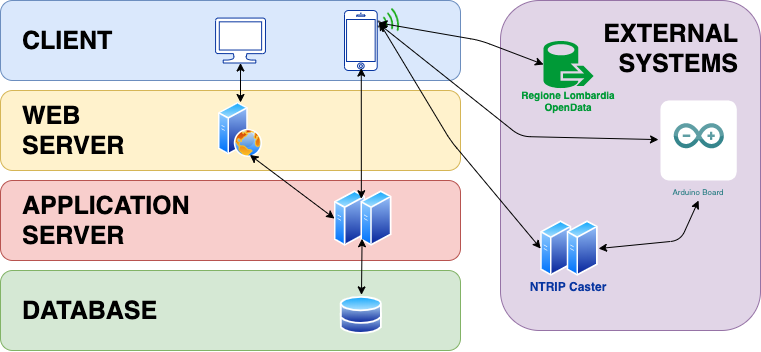
\includegraphics[width=\textwidth]{img/archi/layers.png}
  \hspace{0.05\linewidth}
  \centering
  \caption{\textit{Layered Structure} of the system}
  \label{img:archi_layers}
\end{center}
\end{figure}
\clearpage

The considered high-level components are:
\customParagraph{Mobile Application} 
The \textit{Presentation Layer} dedicated to mobile devices. It communicates with the Application Server to retrieve and send data measured by the \textit{Arduino} board. It contains a wide part of the \textit{Logic Layer} to render data in different ways.\\
The communication with the \textit{Arduino} board is handled with the phone hotspot service; moreover, \textit{Arduino} board could retrieve the RTK GPS correction with a TCP connection with the NTRIPCaster.
  
\customParagraph{Web Browsers}
The \textit{Presentation Layer} dedicated to web browsers; it communicates directly with the Web Server.
  
\customParagraph{Web Server}
It communicates with the Application Server and with the Web Browsers. This is the layer that provides web-pages for the Web Browser; currently, it provides only the SwaggerUI documentation of the RestfulAPI.
  
\customParagraph{Application Server}
This is the layer in which is contained a part of the \textit{Logic Layer} to manage and store users information and collected data with the board; it communicates directly with the Mobile Application, the Web Server and the Database.
  
\customParagraph{Database}
The \textit{Data Layer} of the system; it includes all structures and entities responsible for data storage and management. It communicates with the Application Server.\\\\

In the Figure \ref{img:archi_layers}, \textit{Web Server} and \textit{Application Server} are separated because they represent different function of the application.\\
As mentioned before, it is not implemented a \textit{Web Application} on the \textit{Web Server}, so, in the current setting they are merged.\\ If in future a \textit{Web Application} will be implemented it could be useful to separate the two services in order to allow greater scalability.
\clearpage

\section{Component View}
In this section the system will be described in term of its components:  their functionalities will be discussed and detailed.\\
Moreover, interfaces among components and among external systems will be shown.

\subsection{Database}
The application database is managed using a Relational DBMS. \\
It allows the reading of data, ensuring to the users the possibility to log in, access the application of interest and check the stored data.
It is also used for data manipulation (insertion, modification and deletion).
The use of a Relational DBMS guarantees the fundamental properties for a database of this type:
\begin{itemize}
  \item \textit{Atomicity}: no partial executions of operations;
  \item \textit{Consistency}: the database is always in a consistent state;
  \item \textit{Isolation}: each transaction is executed in an isolated and independent way;
  \item \textit{Durability / Persistence}: changes made are not lost.
\end{itemize}

The database offers to the Application Server an interface that it can use to interact with it.
Particular attention must be paid to the encryption of passwords used to the user access to the system.
Below is the designed E-R diagram (Figure \ref{img:archi_er}).

\begin{figure}[H]
\begin{center}
  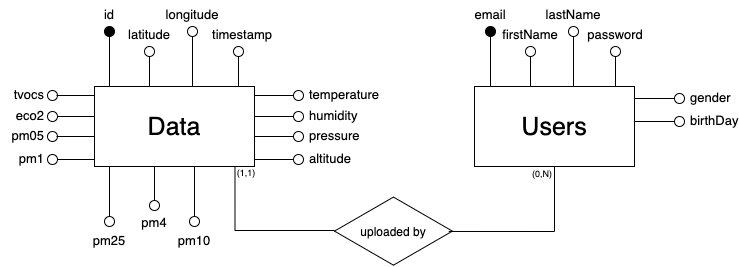
\includegraphics[width=\textwidth]{img/archi/ER.png}
  \hspace{0.05\linewidth}
  \centering
  \caption{\textit{Entity-Relationship} Diagram of the Database}
  \label{img:archi_er}
\end{center}
\end{figure}

\subsection{Application Server}
The main feature of the \textit{Application Server} is to define rules and work-flows of all the functionalities defined by the RestfulAPI.\\
The \textit{Application Server} must have interfaces to communicate with the \textit{Mobile Application} and also with the DBMS; the communication must be done through HTTPS protocol.\\
In the brief introduction below, logic modules and their descriptions are presented, while all the connections among them can be seen in the \textit{Global Component View} in Figure \ref{img:archi_components}.

\customParagraph{Authentication Service}
This module handles the authentication and authorization process. It generates authorization tokens and checks their validity.

\customParagraph{Arduino Data Controller}
This module receives the requests at the \textit{Arduino Data} endpoint, it checks the authorization using the interface with the \textit{Authentication Service} and pass them to the \textit{Arduino Data Service}.

\customParagraph{Arduino Data Service}
This module manages the requests for \textit{Arduino Data} interfacing itself with the \textit{Data Service}.

\customParagraph{Data Service}
This module is the unique interface of the \textit{Application Server} to the database's DBMS.

\customParagraph{User Controller}
This module receives the requests at the \textit{User} endpoint, it checks the authorization using the interface with the \textit{Authentication Service} and pass them to the \textit{User Service}.

\customParagraph{User Service}
This module manages the requests for a \textit{User} interfacing itself with the \textit{Data Service}.

\clearpage
\subsection{Web Server}
As already explained before, the \textit{Web Server} is a simple service. It provides a simple web-page to redirect the user to the \textit{SwaggerUI} documentation.\\
The \textit{Web Server} is hosted in the same space of the \textit{Application Server}; so the connections are done with the HTTPS protocol.\\

\subsection{Mobile Application}
The \textit{MOQA} mobile application communicates with the \textit{Application Server} through RestfulAPIs that are defined in order to describe the interactions between the two layers and that must be independent from the two implementations.\\
The application manages the connection with the \textit{Arduino} board to get air and weather measures and send these data to the \textit{Application Server}. Moreover, it manages the connection with the \textit{Regione Lombardia OpenData} service to retrieve ARPA data.\\

The detailed behaviour of the components in the mobile application is discussed in the Section \ref{sec:ci_mobile}.

\begin{figure}[H]
\begin{center}
  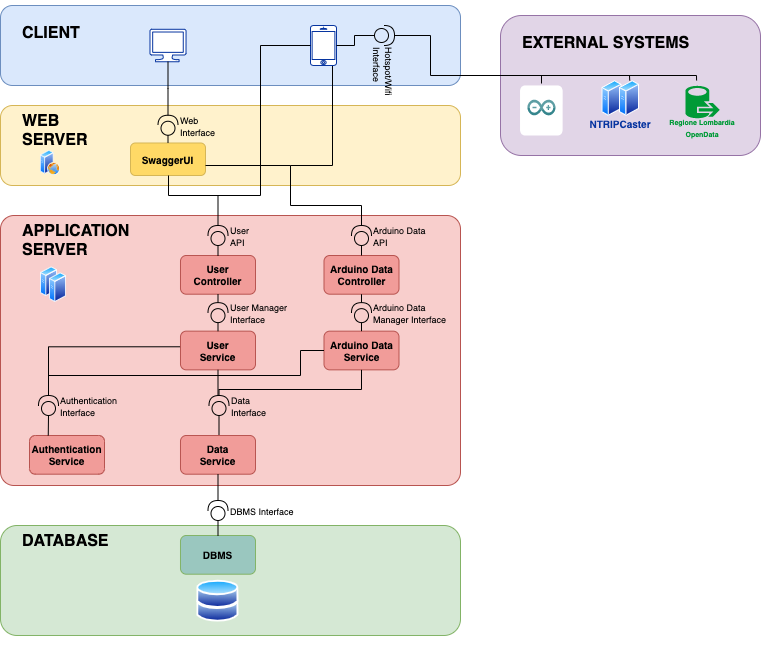
\includegraphics[width=\textwidth]{img/archi/components.png}
  \hspace{0.05\linewidth}
  \centering
  \caption{\textit{Global Component View}}
  \label{img:archi_components}
\end{center}
\end{figure}
\clearpage

\section{Deployment View}
Below is the deployment diagram of the system (Figure \ref{img:archi_deployment}).

\begin{figure}[H]
\begin{center}
  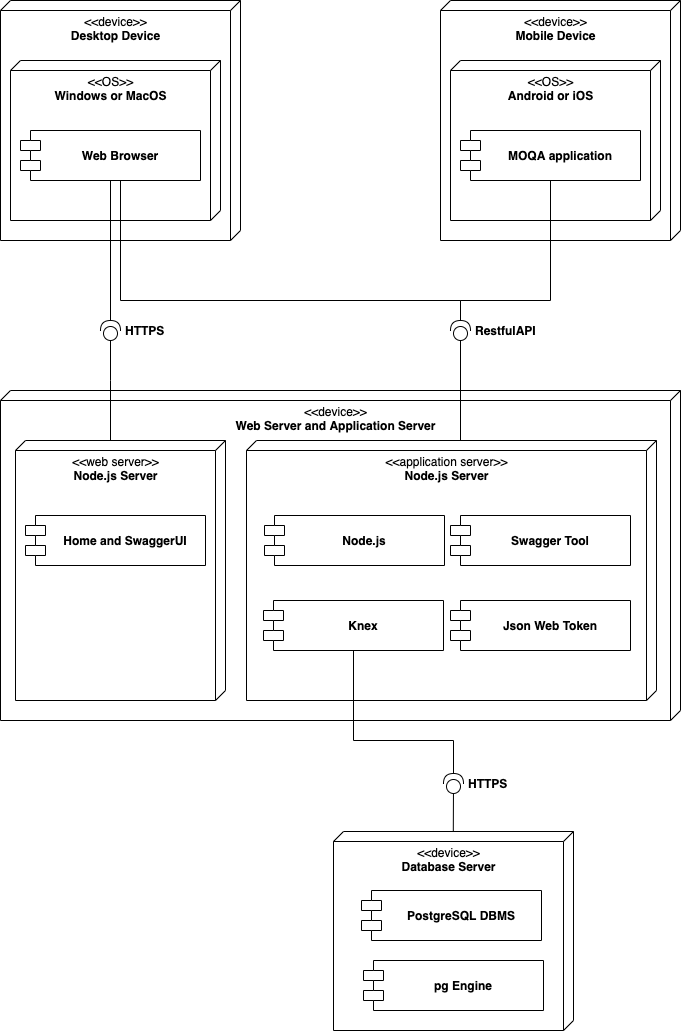
\includegraphics[width=\textwidth,height=.83\textheight,keepaspectratio]{img/archi/deployment.png}
  \hspace{0.05\linewidth}
  \centering
  \caption{\textit{Deployment Diagram} of the system}
  \label{img:archi_deployment}
\end{center}
\end{figure}

\section{Runtime View}\label{sec:runtime}
The aim of this section is to specify the behaviour of the system. Some relevant cases are selected and exploit using \textit{Sequence Diagrams}.

\begin{figure}[H]
\begin{center}
  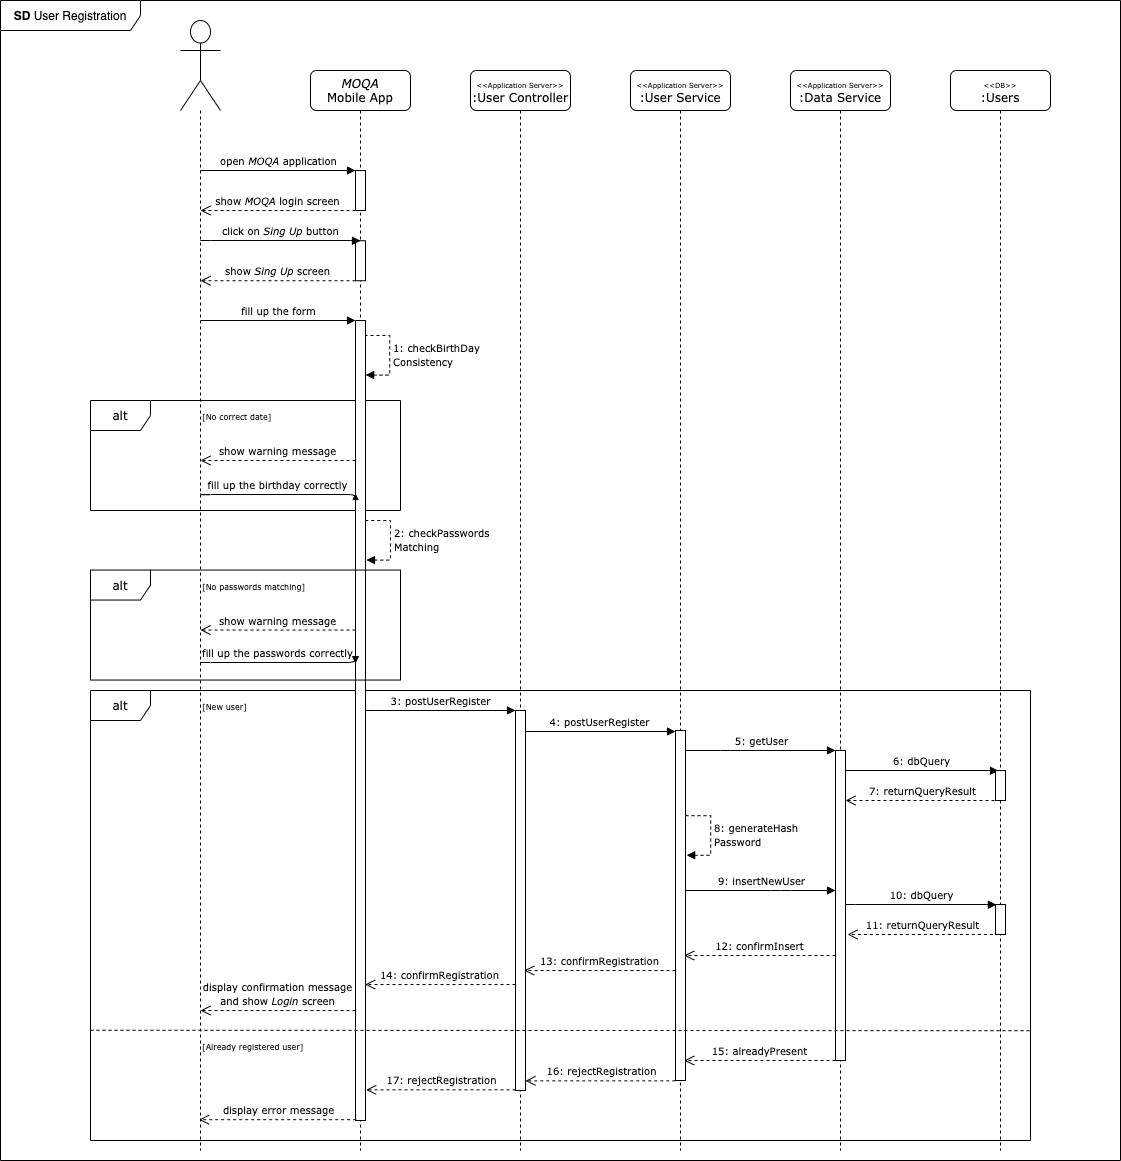
\includegraphics[width=\textwidth,keepaspectratio]{img/archi/sequences/signup.png}
  \hspace{0.05\linewidth}
  \centering
  \caption{\textit{User Signup} sequence diagram: it describes the process through which a user can register itself in the system}
  \label{img:archi_er}
\end{center}
\end{figure}






\section{Component Interfaces}
This section contains some detailed information about the interfaces between the components of the system.\\
The following description focuses the attention over the actions performed by a procedure of a certain component after that it is called by other components.\\
Huge part of these actions could be seen played in the \textit{Sequence Diagrams} (Section \ref{sec:runtime}).

\subsection{Application Server}

\customParagraph{Authentication Service}
Following procedures are called by other components:
\begin{itemize}
    \item \textbf{generateJWT}\quad This method allows to generate a token for the authentication. The token must be added in the requests as \textit{Header} attribute.
    \item \textbf{decodeJWT}\quad This method allows to get and decode the token, if present, in a request. It returns the object with the information of the.
\end{itemize}

\customParagraph{Arduino Data Controller}
Following procedures are called by other components:
\begin{itemize}
    \item \textbf{getData}\quad This method is called when a request is received at the corresponding endpoint. It calls the \textit{Authentication Service} to check the session. If the session is valid, it retrieves the parameters in the request and calls the corresponding method in the \textit{Arduino Data Service}.
    \item \textbf{getDataByDate}\quad This method is called when a request is received at the corresponding endpoint. It calls the \textit{Authentication Service} to check the session. If the session is valid, it retrieves the parameters in the request and calls the corresponding method in the \textit{Arduino Data Service}.
    \item \textbf{postData}\quad This method is called when a request is received at the corresponding endpoint. It calls the \textit{Authentication Service} to check the session. If the session is valid, it retrieves the parameters in the request and calls the corresponding method in the \textit{Arduino Data Service}.
\end{itemize}

\customParagraph{Arduino Data Service}
Following procedures are called by other components:
\begin{itemize}
    \item \textbf{getData}\quad This method is called by the \textit{Arduino Data Controller}. It retrieves the data preparing the query to submit to the \textit{Data Service}.
    \item \textbf{getDataByDate}\quad This method is called by the \textit{Arduino Data Controller}. It retrieves the data preparing the query to submit to the \textit{Data Service}
    \item \textbf{postData}\quad This method is called by the \textit{Arduino Data Controller}. It retrieves the data preparing the query to submit to the \textit{Data Service}
\end{itemize}

\customParagraph{Data Service}
Following procedure is called by other components:
\begin{itemize}
    \item \textbf{databaseInit}\quad This method is called during the initialization of the \textit{Application Server} to create the tables in the database and initialize them with the initials data.
\end{itemize}

Moreover, it provides an object that has own methods to query the database through the DBMS service.

\customParagraph{User Controller}
Following procedures are called by other components:
\begin{itemize}
    \item \textbf{deleteUserMe}\quad This method is called when a request is received at the corresponding endpoint. It calls the \textit{Authentication Service} to check the session, if the session is valid it retrieves, from the session, the user email and calls the corresponding method in the \textit{Arduino Data Service}.
    \item \textbf{getUserMe}\quad This method is called when a request is received at the corresponding endpoint. It calls the \textit{Authentication Service} to check the session, if the session is valid it retrieves, from the session, the user email and calls the corresponding method in the \textit{Arduino Data Service}.
    \item \textbf{postUserLogin}\quad This method is called when a request is received at the corresponding endpoint. It retrieves the parameters in the request and calls the corresponding method in the \textit{Arduino Data Service}.
    \item \textbf{postUserLogout}\quad This method is called when a request is received at the corresponding endpoint. It calls the \textit{Authentication Service} to check the session, if the session is valid it logout the user.
    \item \textbf{postUserRegister}\quad This method is called when a request is received at the corresponding endpoint. It retrieves the parameters in the request and calls the corresponding method in the \textit{Arduino Data Service}.
    \item \textbf{putUserMe}\quad This method is called when a request is received at the corresponding endpoint. It calls the \textit{Authentication Service} to check the session. If the session is valid, it retrieves the parameters in the request, checks the consistency* and calls the corresponding method in the \textit{Arduino Data Service}.
\end{itemize}

*: the consistency is computed checking if the session email is the same in the body in the PUT request.

\customParagraph{User Service}
Following procedures are called by other components:
\begin{itemize}
    \item \textbf{deleteUserMe}\quad This method is called by the \textit{User Controller}. It retrieves the data preparing the query to submit to the \textit{Data Service}.
    \item \textbf{getUserMe}\quad This method is called by the \textit{User Controller}. It retrieves the data preparing the query to submit to the \textit{Data Service}.
    \item \textbf{postUserLogin}\quad This method is called by the \textit{User Controller}. It retrieves the data preparing the query to submit to the \textit{Data Service}.
    \item \textbf{postUserRegister}\quad This method is called by the \textit{User Controller}. It retrieves the data preparing the query to submit to the \textit{Data Service}.
    \item \textbf{putUserMe}\quad This method is called by the \textit{User Controller}. It retrieves the data preparing the query to submit to the \textit{Data Service}.
\end{itemize}

\subsection{Mobile Application}\label{sec:ci_mobile}


\section{Architecture styles and patterns}
\clearpage

% UI Design
\chapter{User Interface Design}
\section{Overview}
In this section are present some screenshots by \textit{MOQA} mobile application.\\
During the design and development, the attention was focused on the mobile application, even if the application is developed to adapt itself to a larger screen. Layout, dimensions and colours are picked by the Apple Human Interface Guidelines.\\

\section{Mock-up}
At the beginning of the project, it was provided to the stakeholders a \textit{mock-up} (Figure \ref{img:initialWireframe}) of the application to have an approval that the draft was meeting the requirements and to show an overview of the flow of the application.

\begin{figure}[H]
\begin{center}
  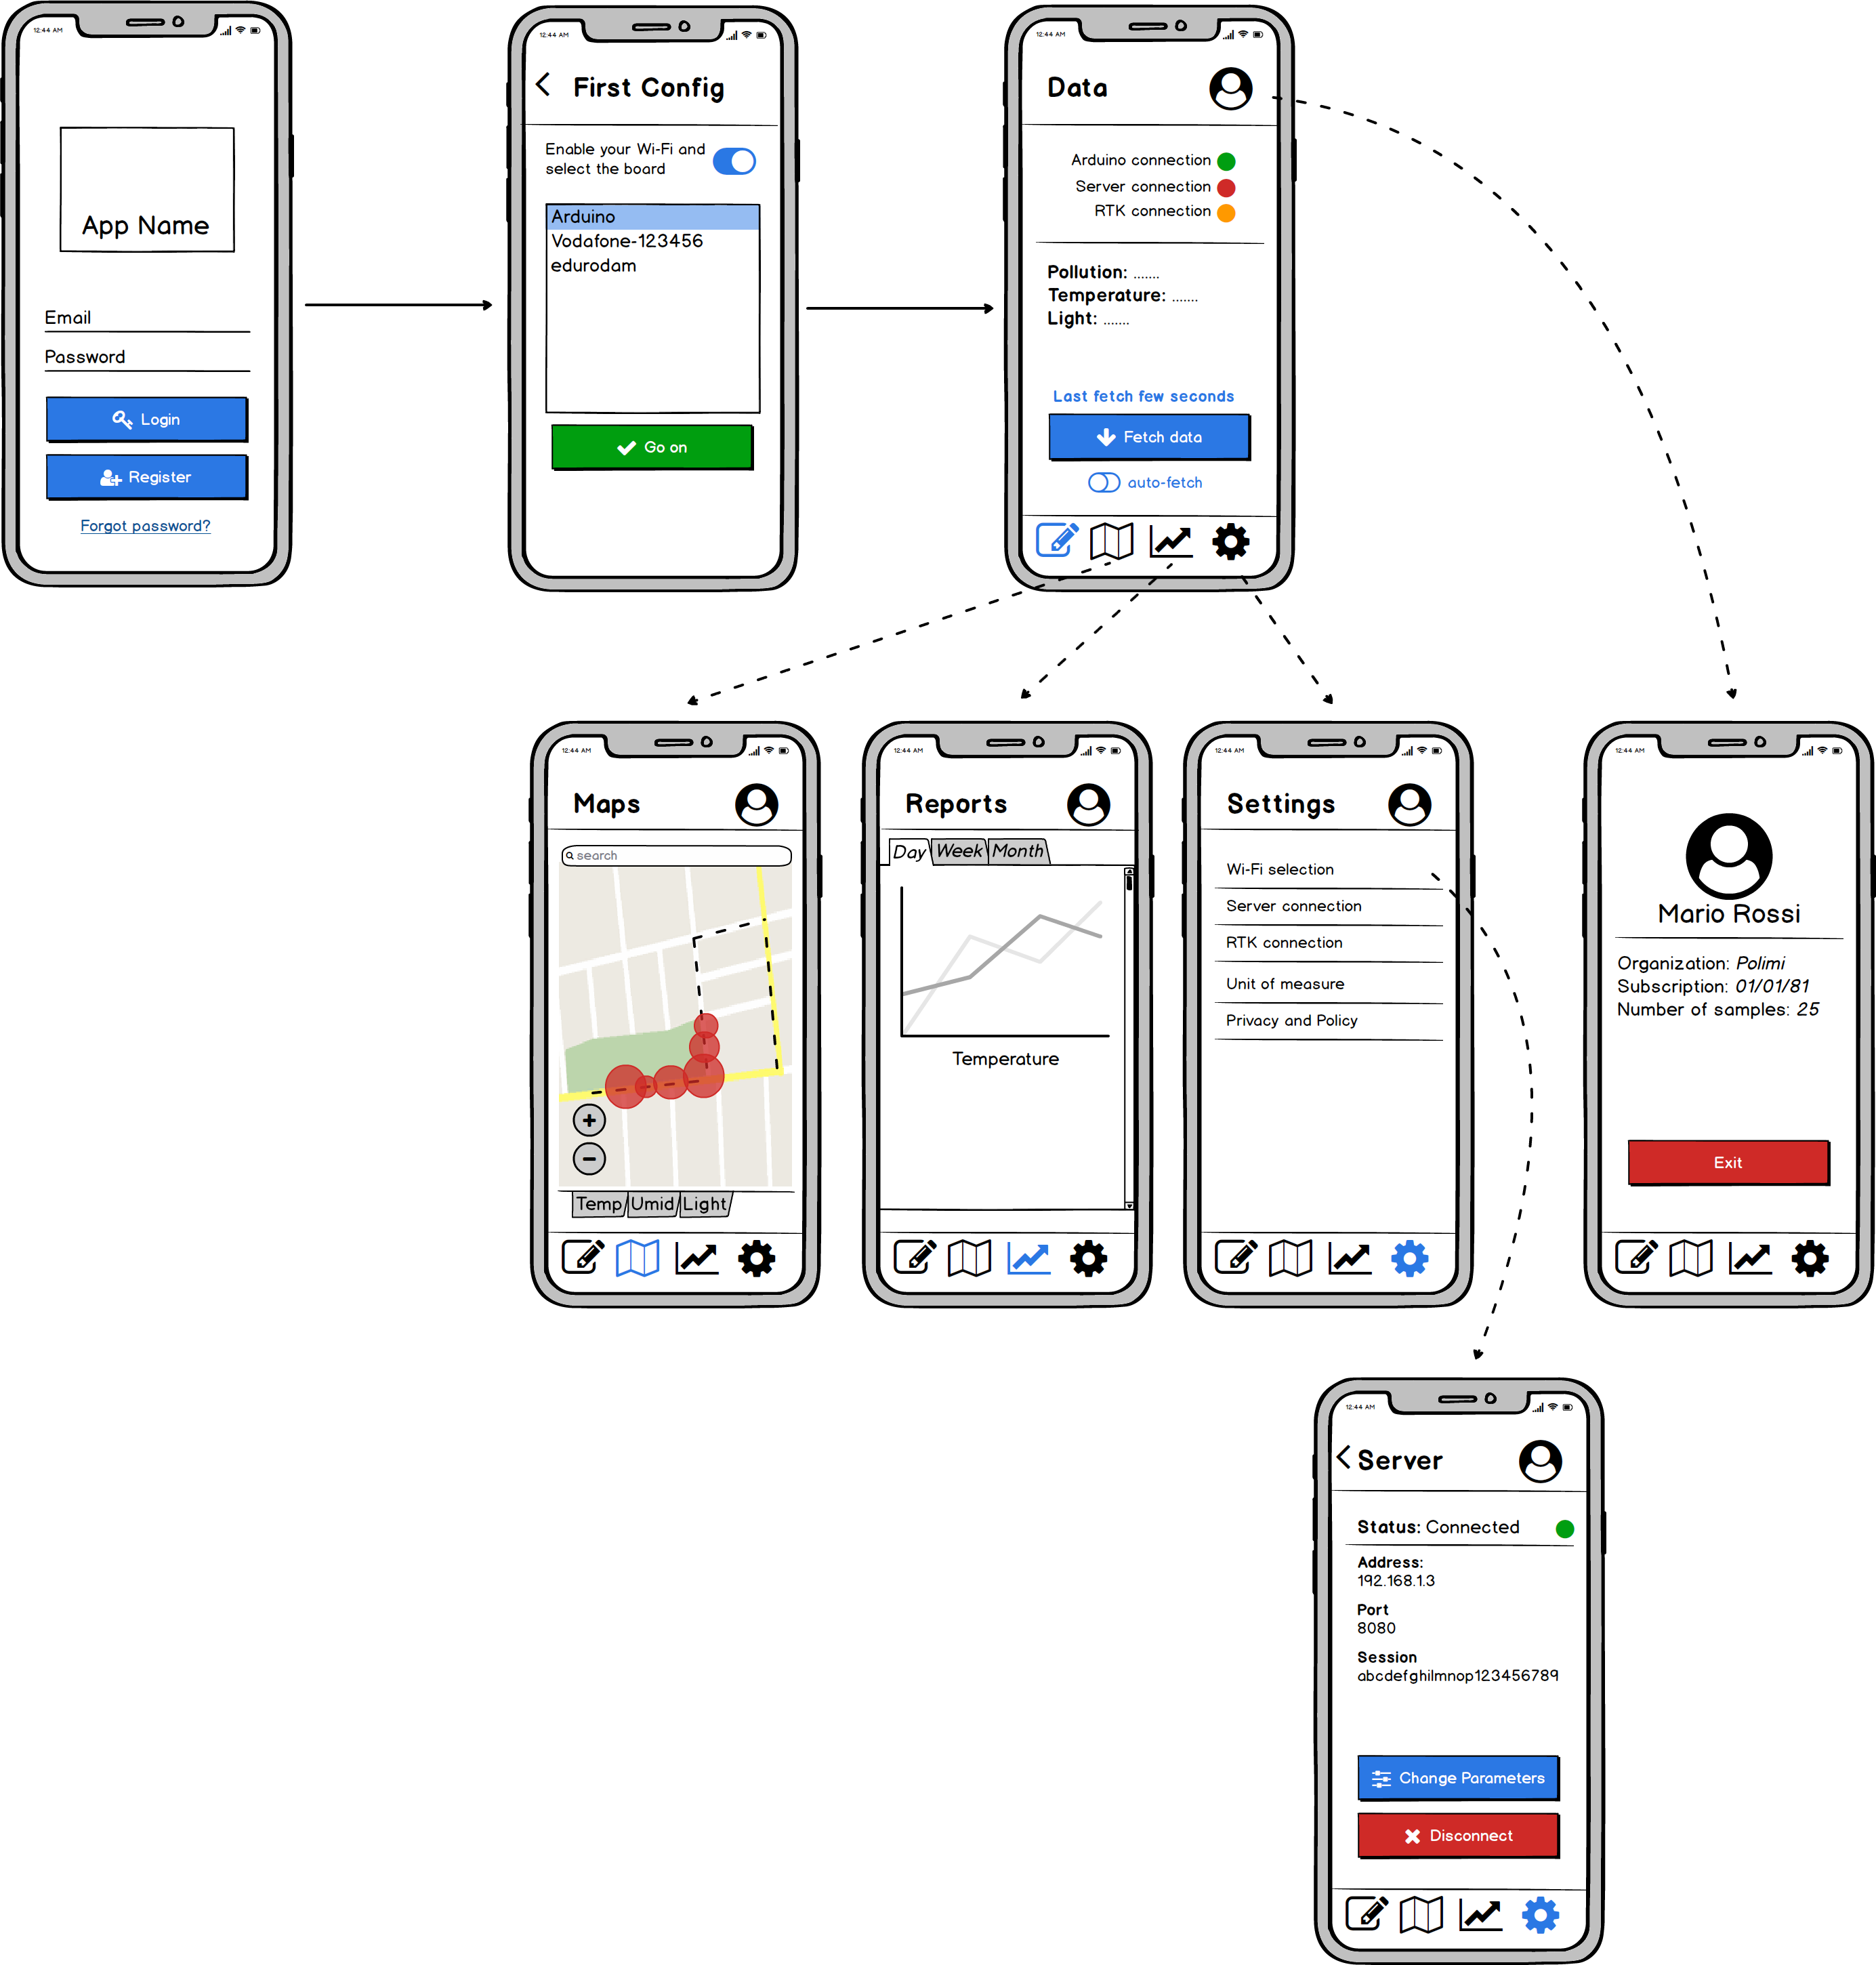
\includegraphics[width=\textwidth]{img/initialWireframe.png}
  \hspace{0.05\linewidth}
  \centering
  \caption{\textit{MOQA} initial mock-up}
  \label{img:initialWireframe}
\end{center}
\end{figure}
\clearpage

\section{Screens}

\begin{figure}[H]
\centering
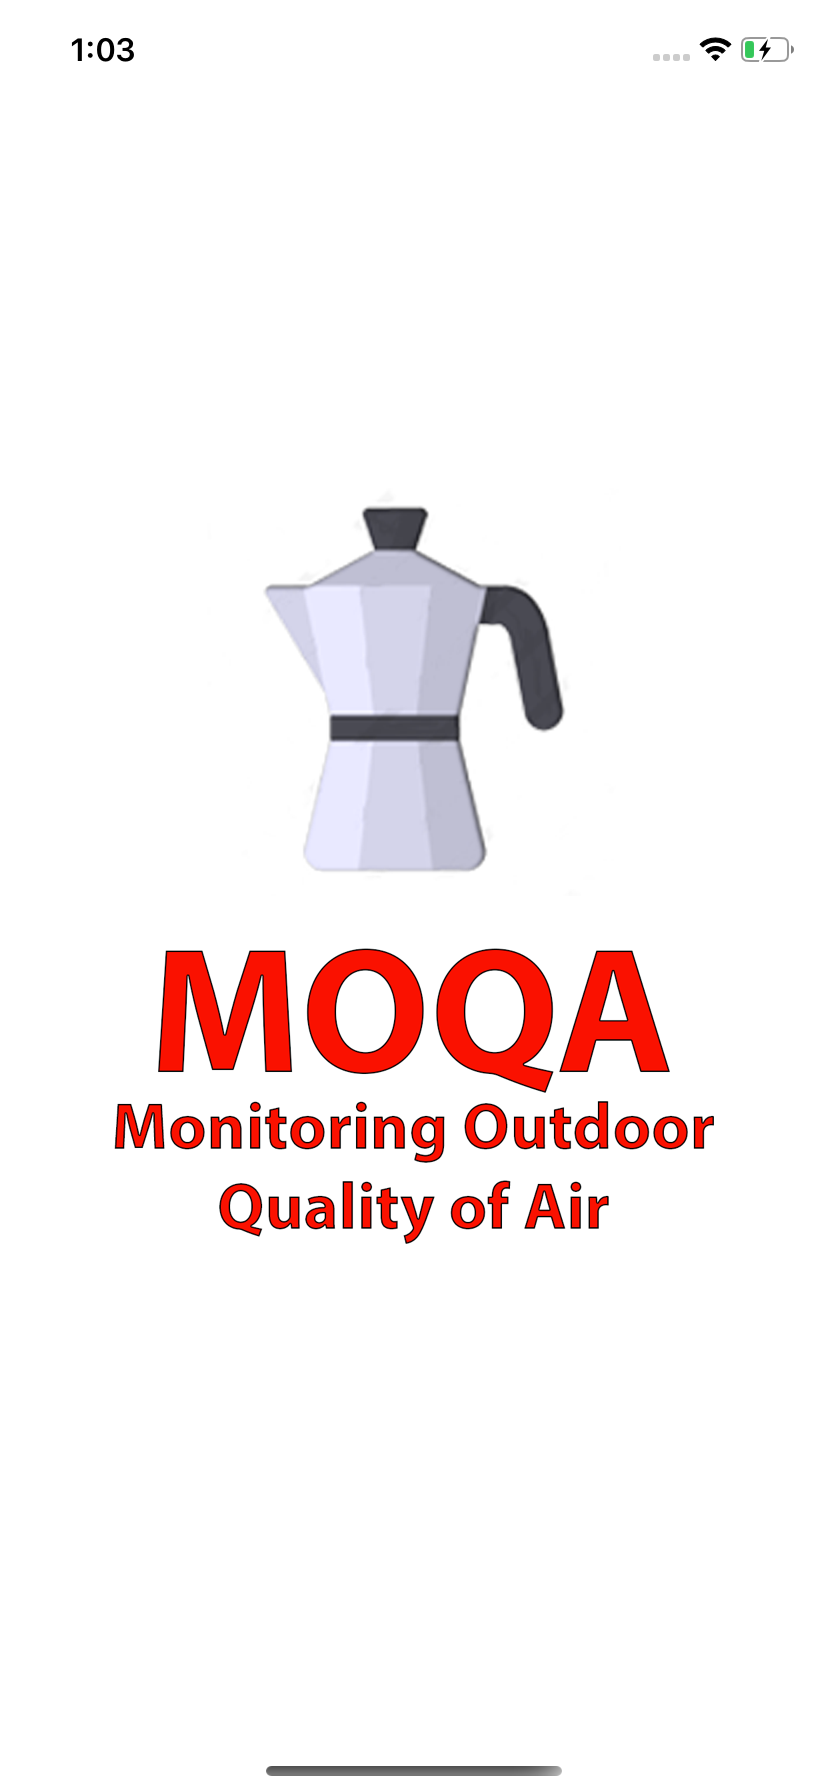
\includegraphics[height=.6\textheight]{./img/ui/splash.png}
\caption{\textbf{Splash Screen}}
\end{figure}
\begin{center}
The \textbf{Splash Screen} welcomes the user when the application is starting; meanwhile it restores the state of the application or loads the default one.    
\end{center}

\begin{figure}[H]
\centering
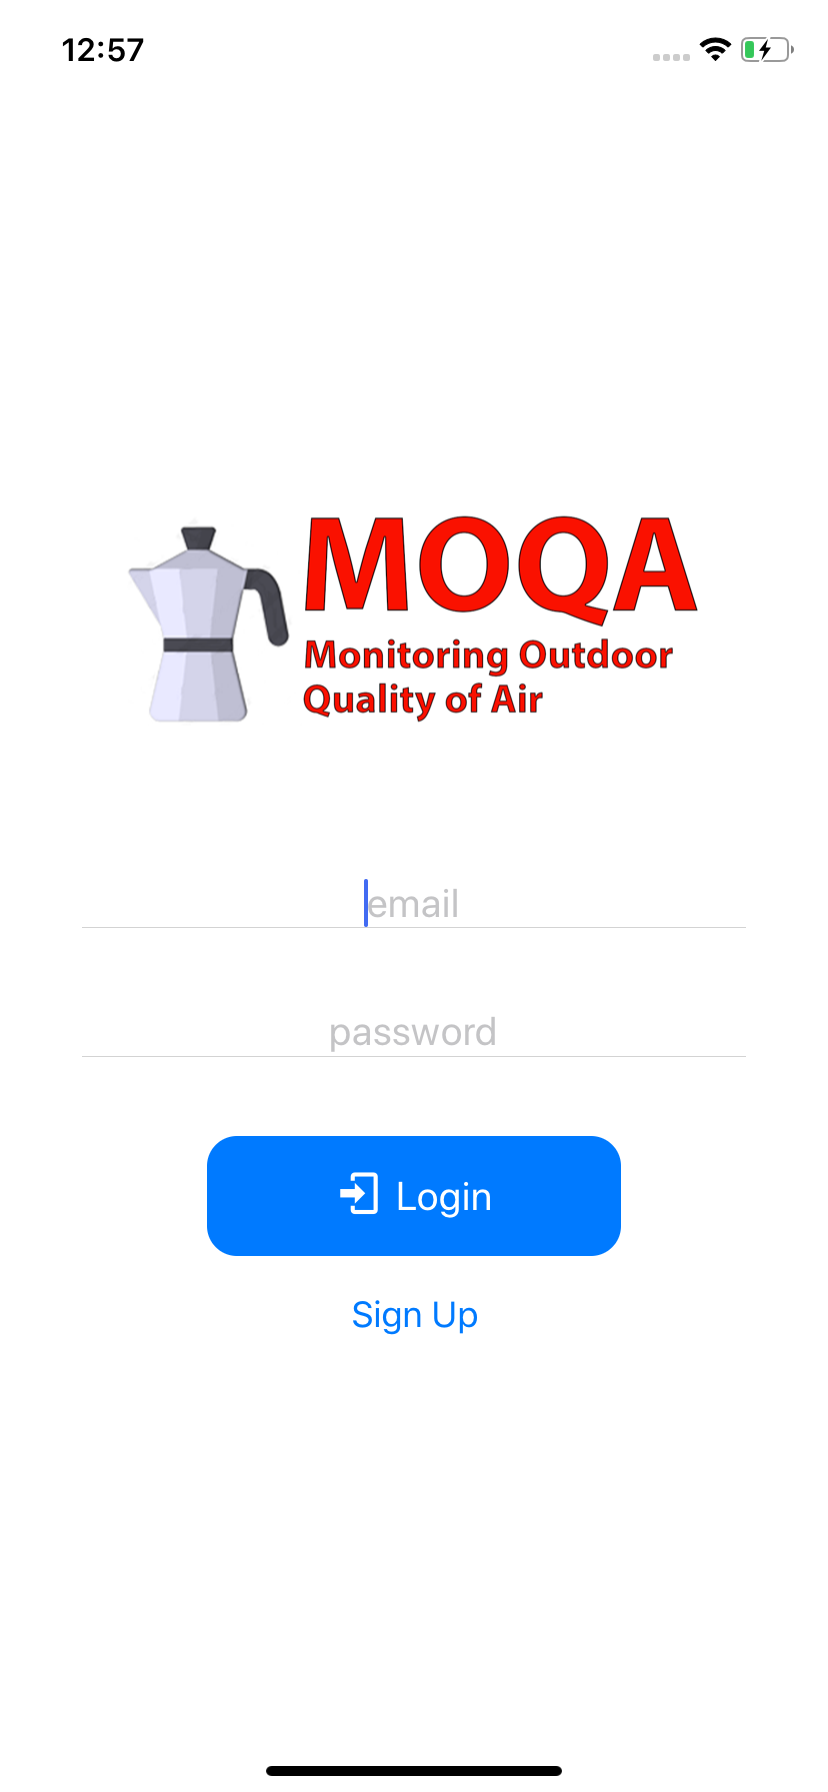
\includegraphics[height=.6\textheight]{./img/ui/login.png}
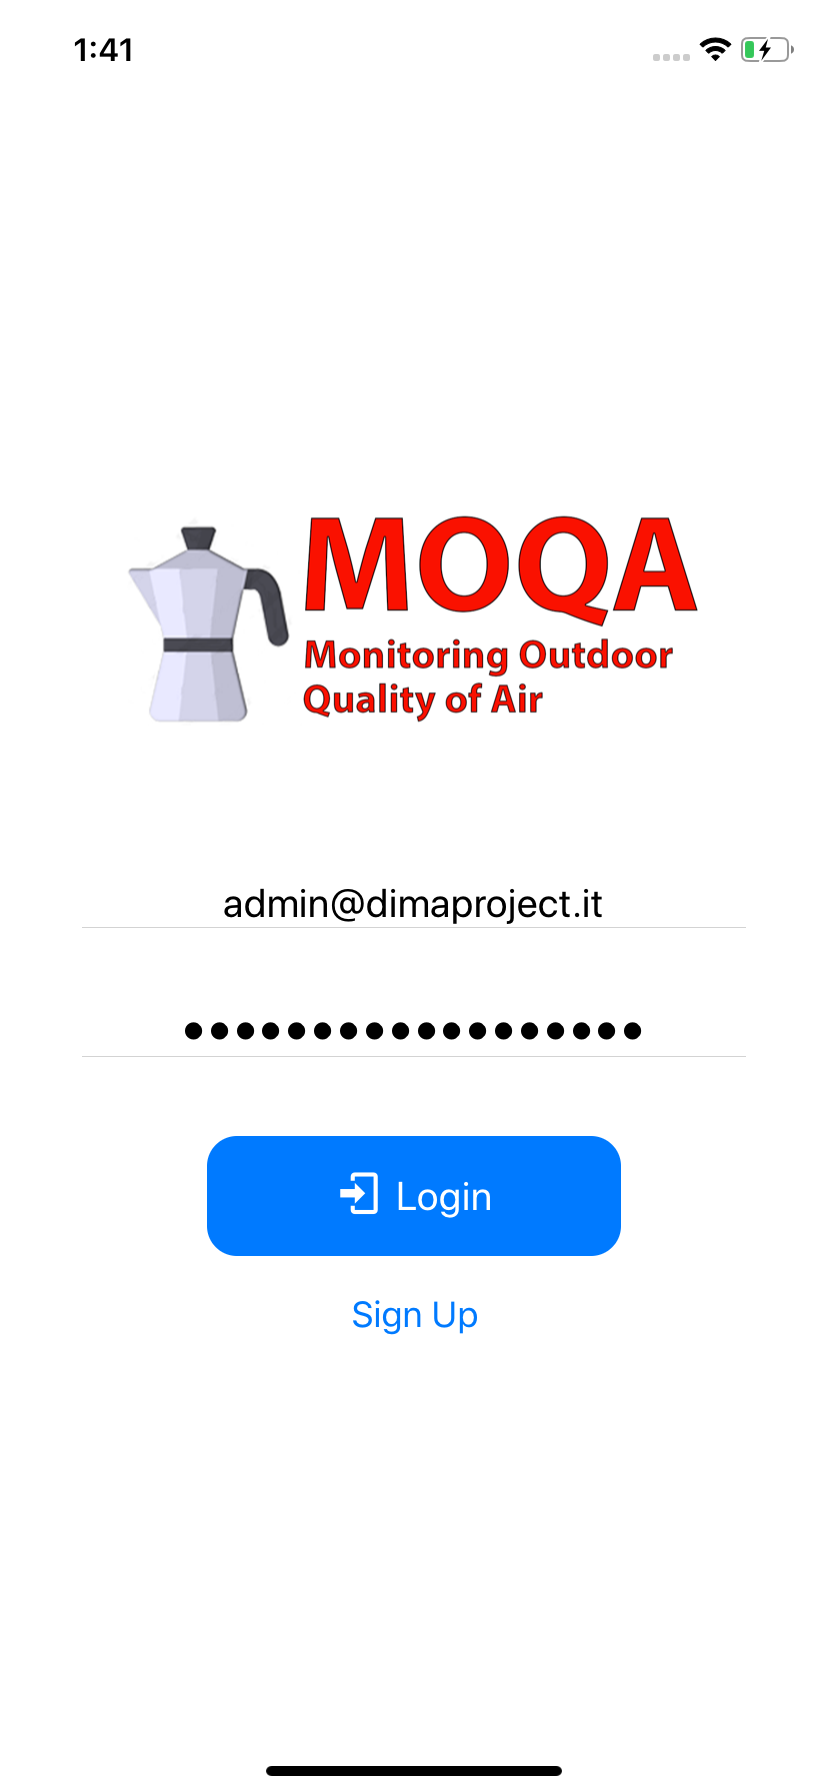
\includegraphics[height=.6\textheight]{./img/ui/login2.png}
\caption{\textbf{Login Screen}}
\end{figure}
\begin{center}
The \textbf{Login Screen} is the first screen that the user sees after the application is loaded. The user could enter its credential or, if they are in memory, the application fills the fields.
\end{center}

\begin{figure}[H]
\centering
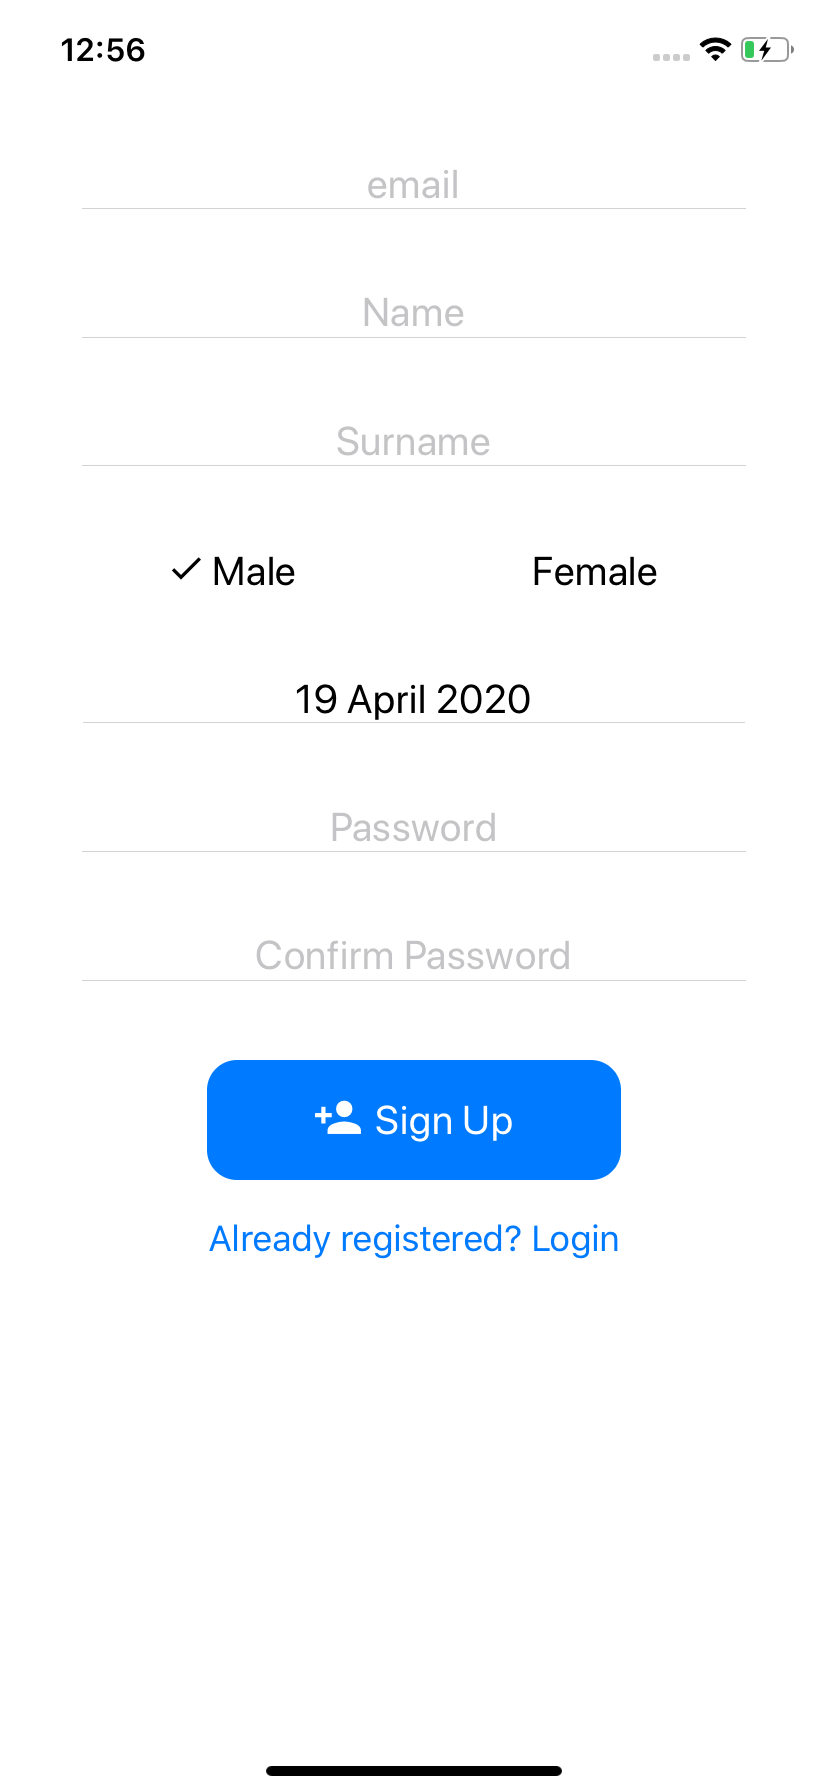
\includegraphics[height=.6\textheight]{./img/ui/signup.png}
\caption{\textbf{Sign Up Screen}}
\end{figure}
\begin{center}
The \textbf{Sign Up Screen} allows the user to register in the application.
\end{center}

\begin{figure}[H]
\centering
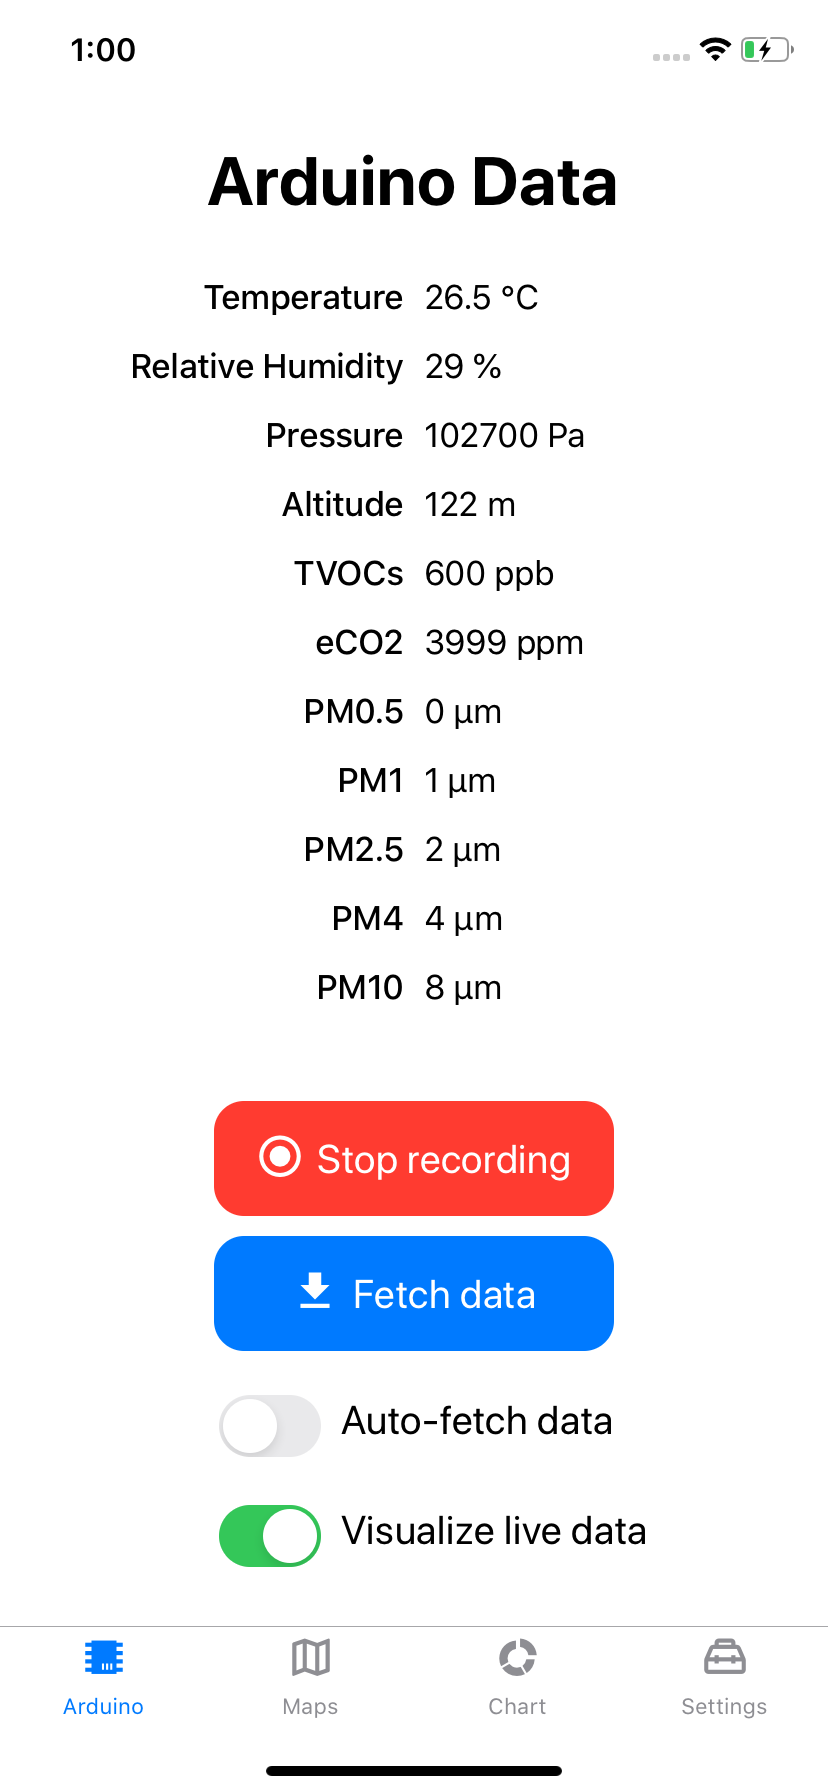
\includegraphics[height=.6\textheight]{./img/ui/arduino_data.png}
\caption{\textbf{Arduino Screen}}
\end{figure}
\begin{center}
The \textbf{Arduino Screen} displays the data coming from the \textit{Arduino} board, if available.\\
It allows the user to start/stop the recording of data (it means that the data gathered by the board are sent to the server).\\
It allows the user to \textit{Fetch data} (it is a manual request of data to the board) or enable the \textit{Auto-fetch data} that starts a routine that every second refreshes the data from the board.\\
Moreover in this screen, the user could decide if it wants to visualize the live data from the board or the data stored in the server in the \textbf{Map Screen} and \textbf{Chart Screen}.
\end{center}

\begin{figure}[H]
\centering
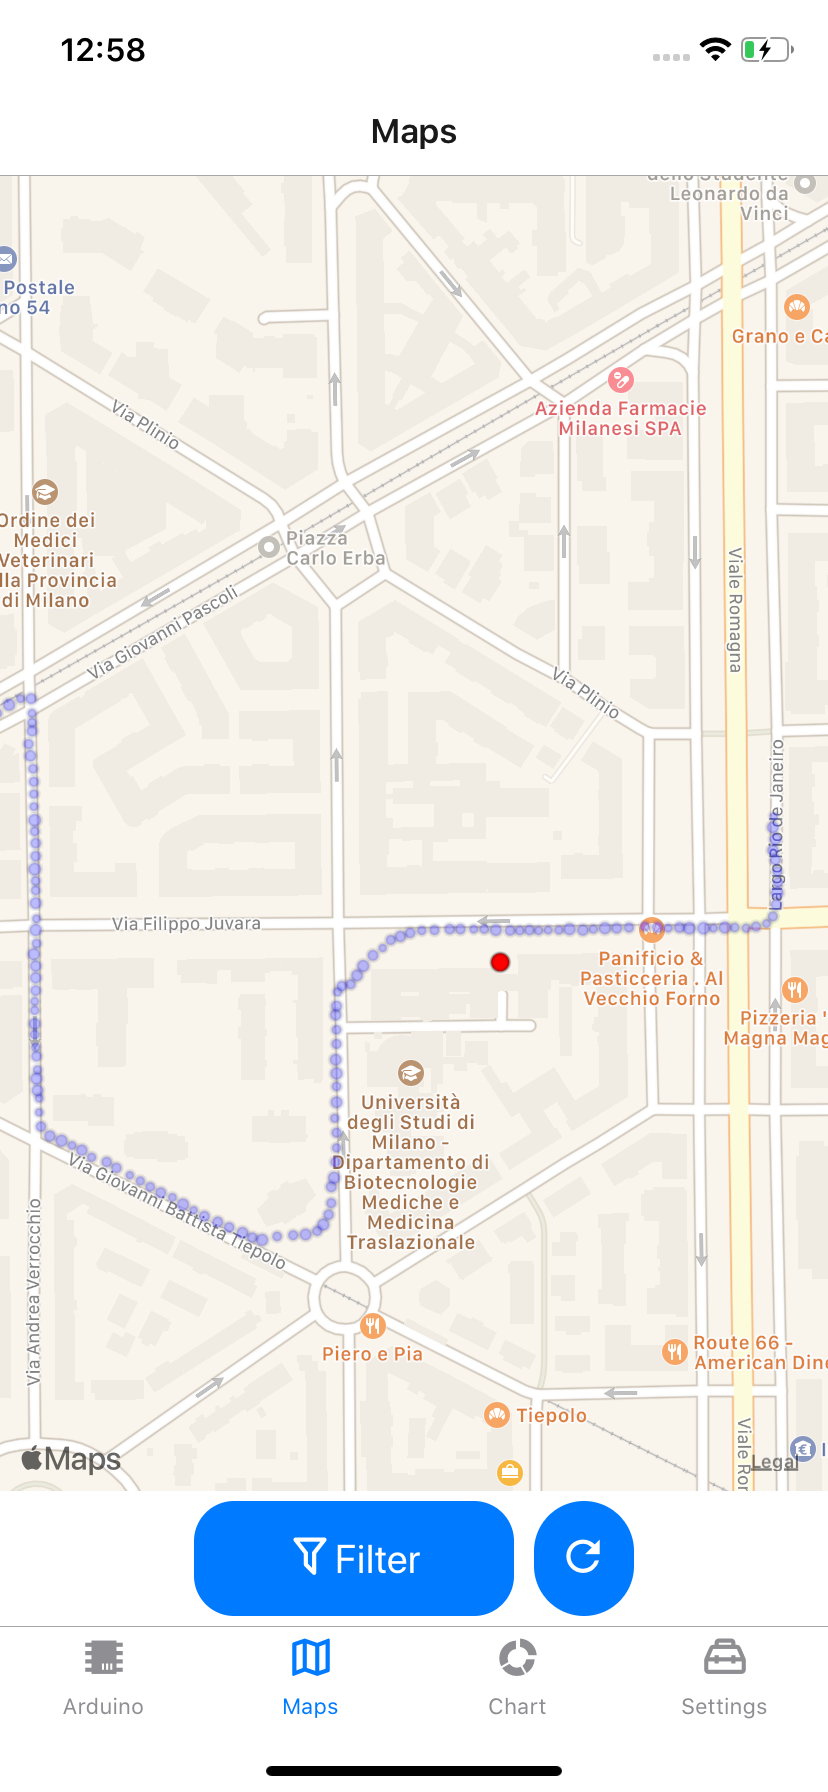
\includegraphics[height=.6\textheight]{./img/ui/map.png}
\caption{\textbf{Map Screen}}
\end{figure}
\begin{center}
The \textbf{Map Screen} displays the data coming from the \textit{Arduino} board (blue circles) and \textit{ARPA} dataset (red circles) on a map. The radius of a circle depends on the value of the data it is associated.\\
The user could filter the data clicking on the \textit{Filter} button and could refresh the map with the blue button on the right.
\end{center}

\begin{figure}[H]
\centering
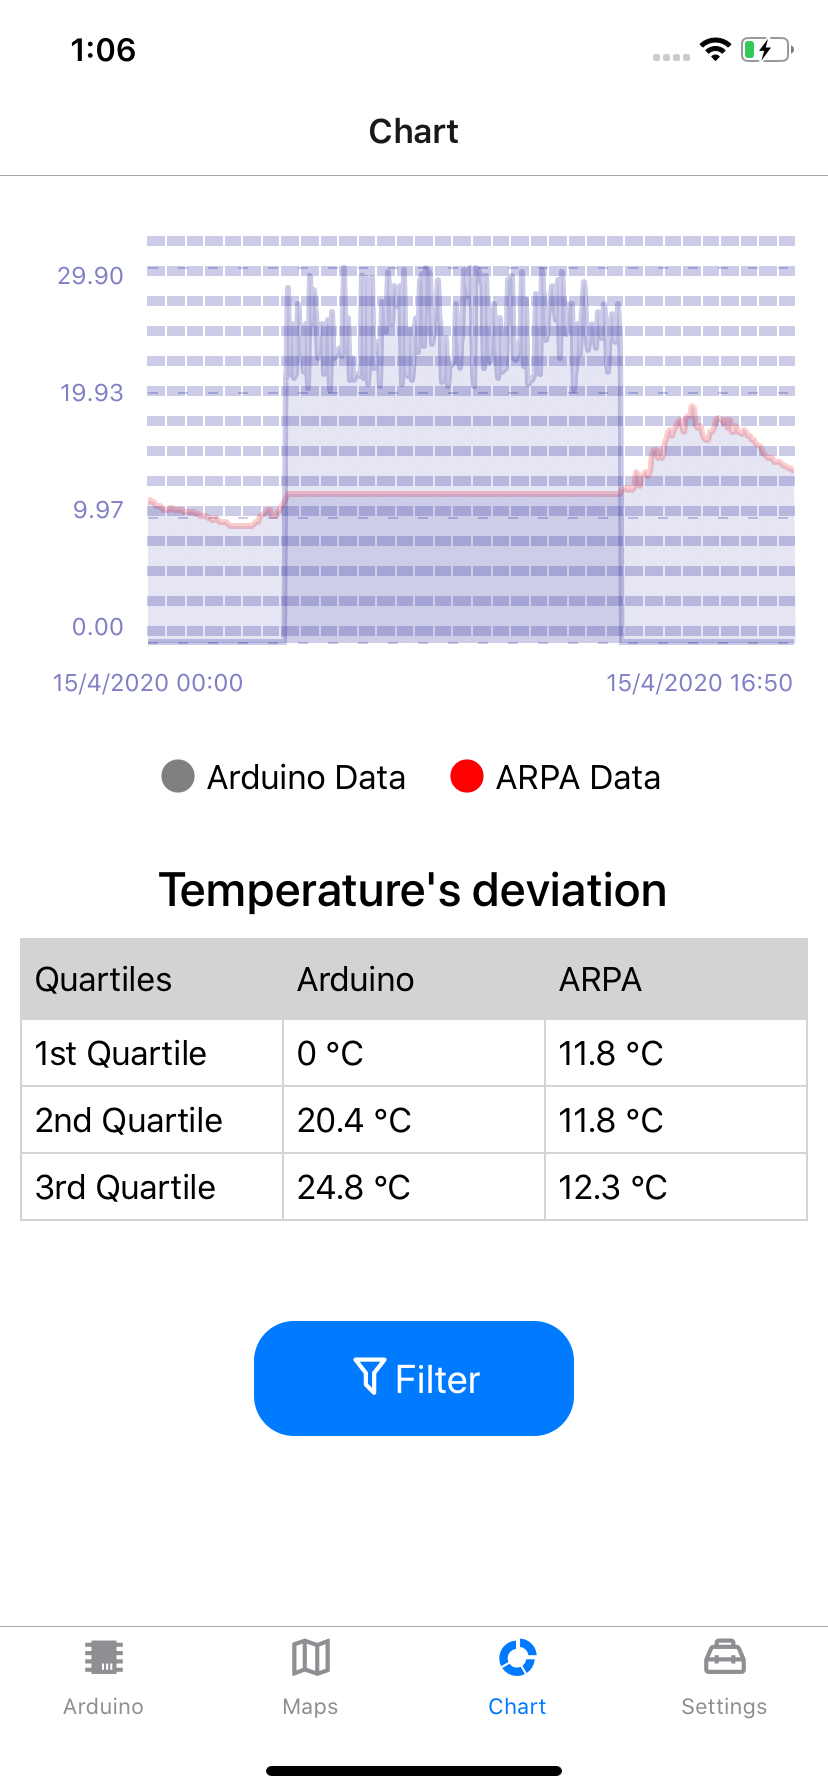
\includegraphics[height=.6\textheight]{./img/ui/chart.png}
\caption{\textbf{Chart Screen}}
\end{figure}
\begin{center}
The \textbf{Chart Screen} displays the data coming from the \textit{Arduino} board and \textit{ARPA} dataset on a graph. Moreover, it provides a table with a computation of the quartile deviation.\\
The user could filter the data clicking on the \textit{Filter} button and could refresh the page scrolling-up.
\end{center}

\begin{figure}[H]
\centering
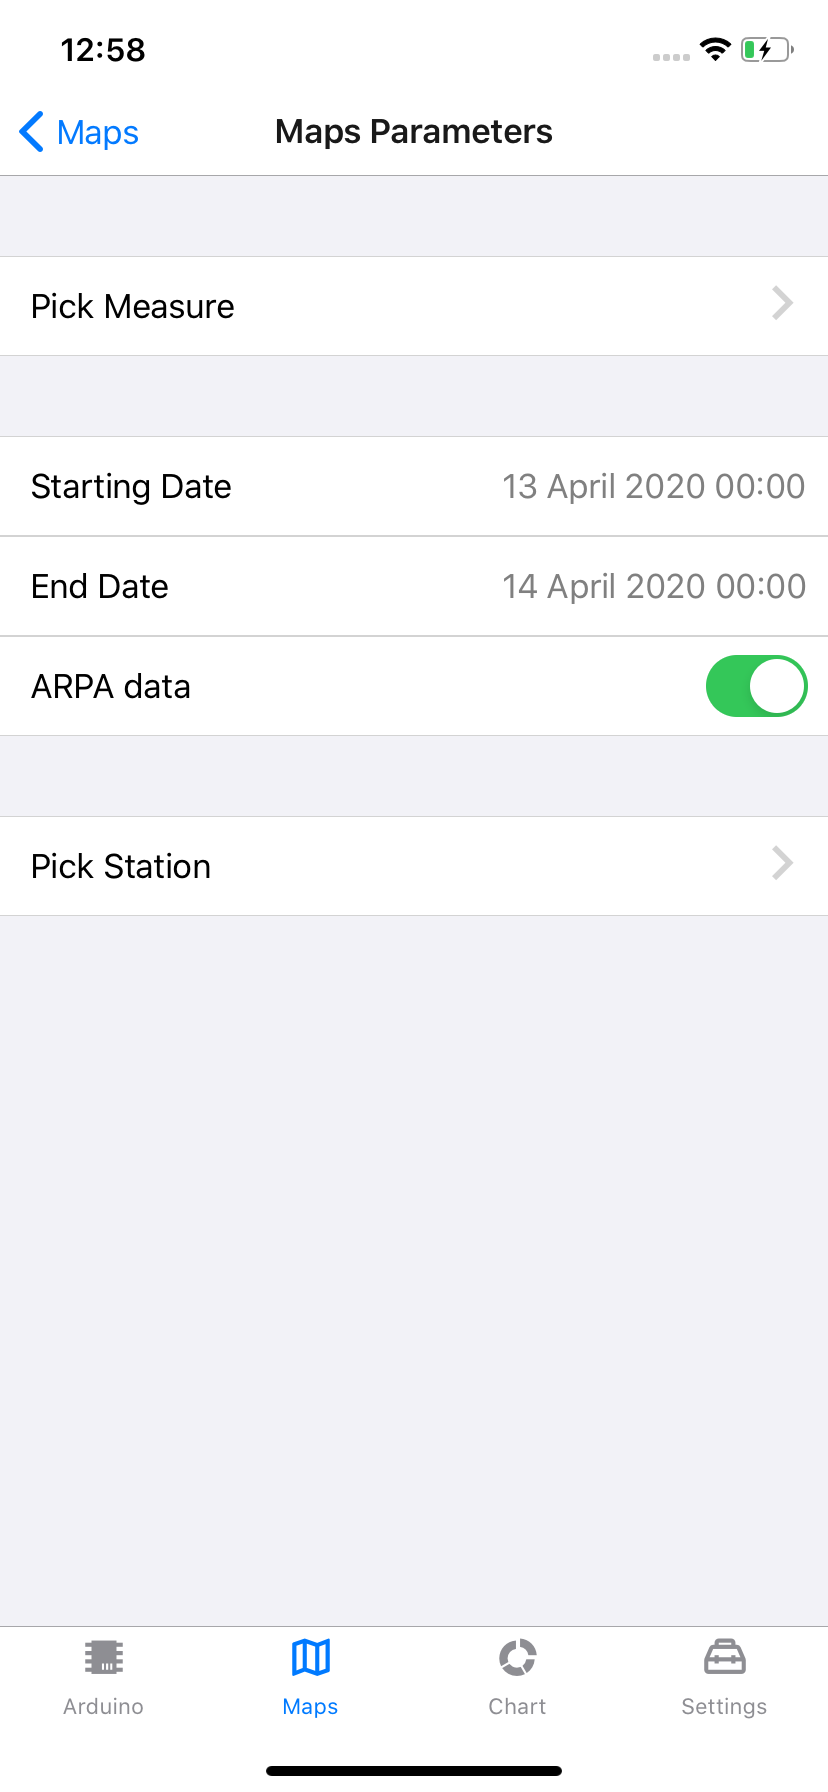
\includegraphics[height=.6\textheight]{./img/ui/filter.png}
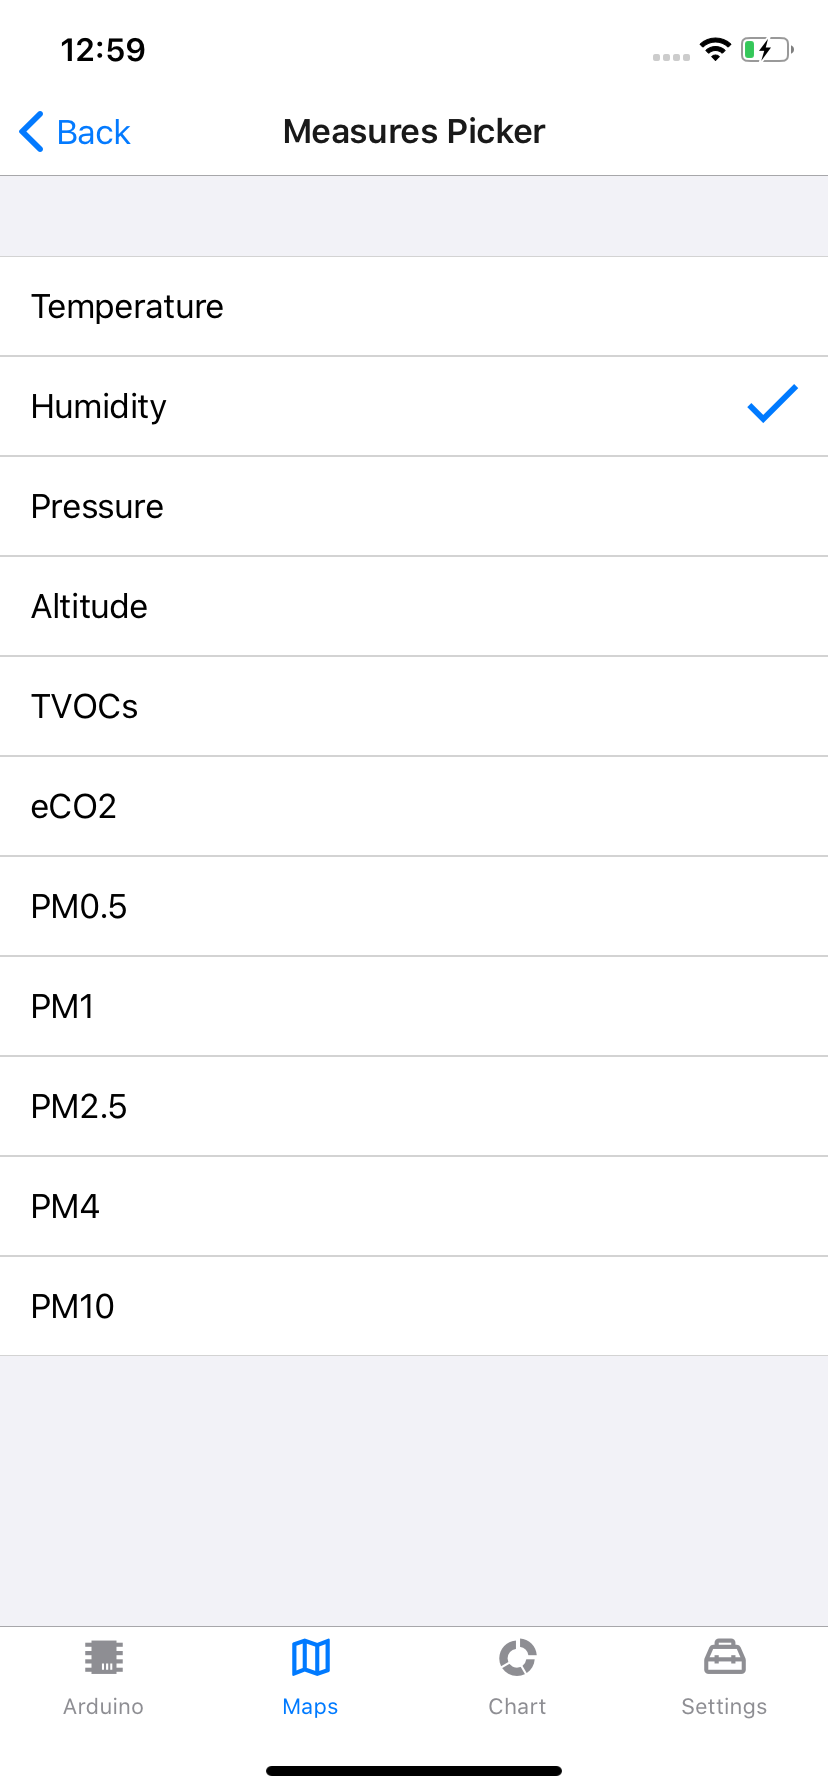
\includegraphics[height=.6\textheight]{./img/ui/mea_picker.png}
\caption{\textbf{Filter Screens}}
\end{figure}
\begin{center}
The \textbf{Filter Screens} allow the user to set the parameters to limit the data visualized in the \textbf{Map Screen} and \textbf{Chart Screen}.\\
The user could pick the measure it wants to visualize, select the time range and decide to visualize the ARPA data defining the station.\\
In the application the \textbf{Filter Screen} is used by the \textbf{Map Screen} and the \textbf{Chart Screen}
\end{center}

\begin{figure}[H]
\centering
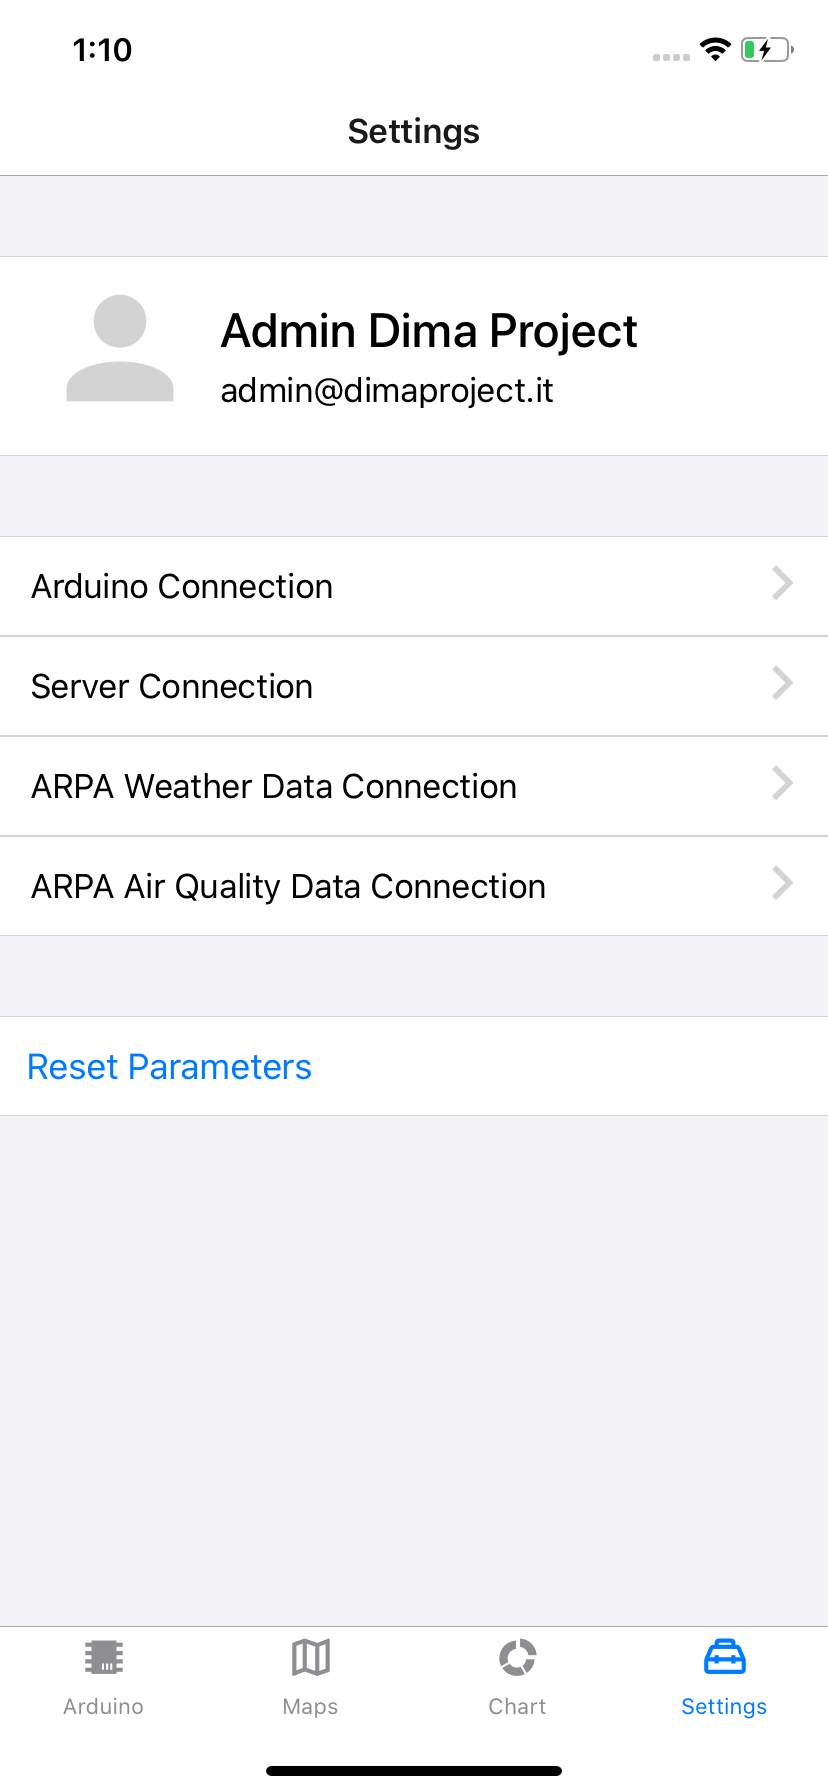
\includegraphics[height=.6\textheight]{./img/ui/settings.png}
\caption{\textbf{Settings Screen}}
\end{figure}
\begin{center}
The \textbf{Settings Screen} allows the user to visualize and to change different parameters of the application.\\
The user could also decide to reset the parameters to an initial and default state.
\end{center}

\begin{figure}[H]
\centering
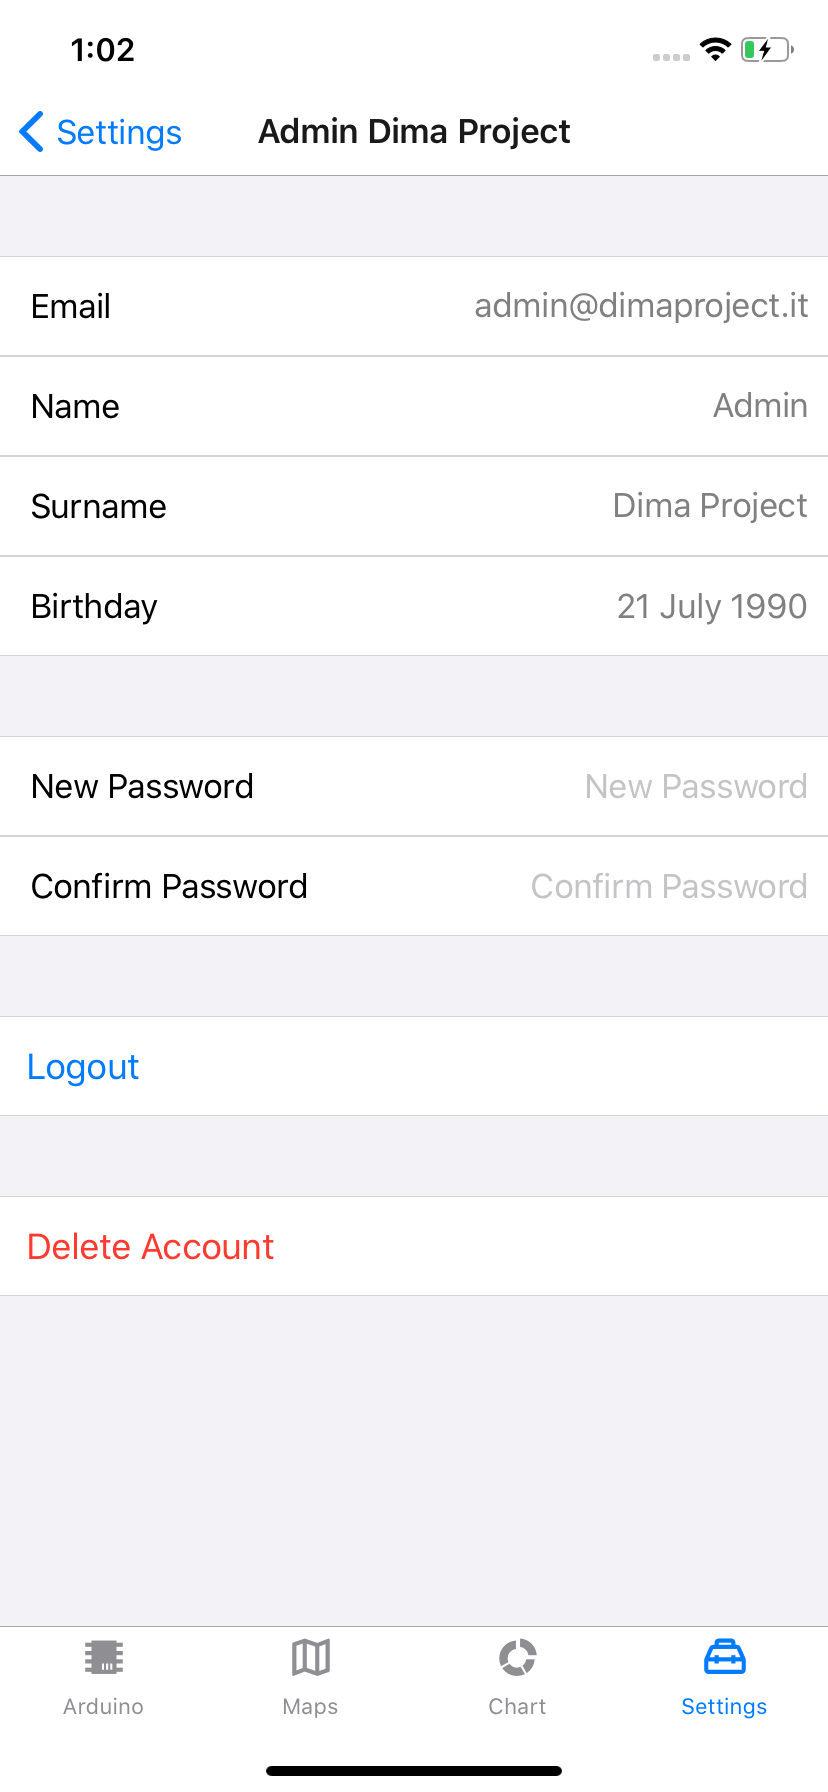
\includegraphics[height=.6\textheight]{./img/ui/user_settings.png}
\caption{\textbf{User Settings Screen}}
\end{figure}
\begin{center}
The \textbf{User Settings Screen} allows the user to visualize and to change the information about its account. Moreover it allows the user to delete its account or logout from the application.
\end{center}

\begin{figure}[H]
\centering
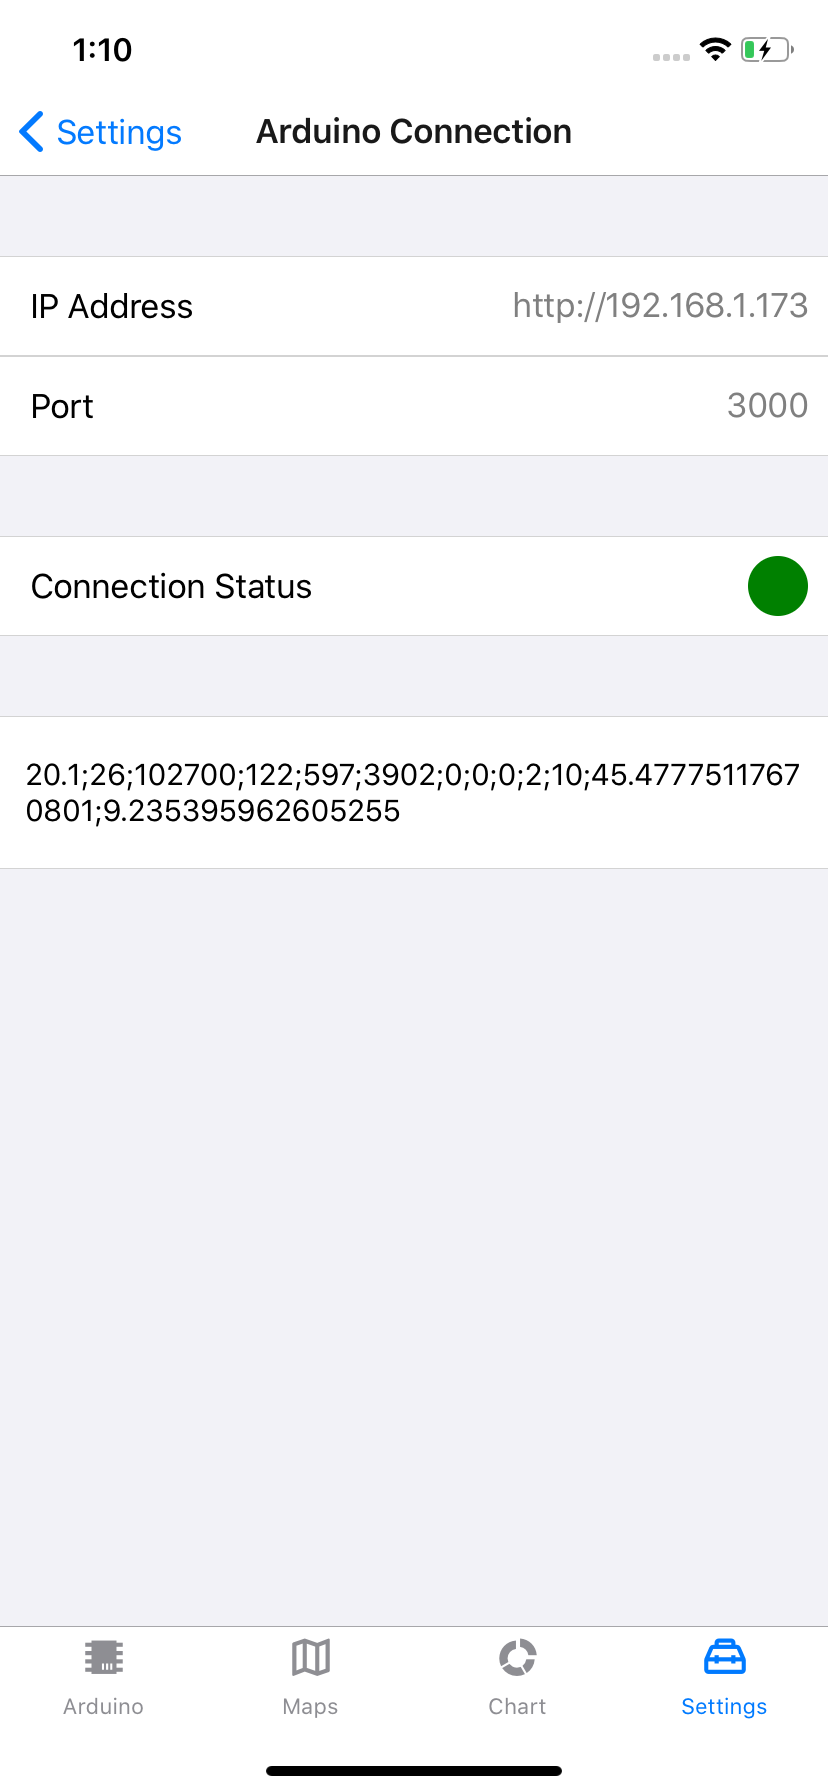
\includegraphics[height=.6\textheight]{./img/ui/arduino_settings.png}
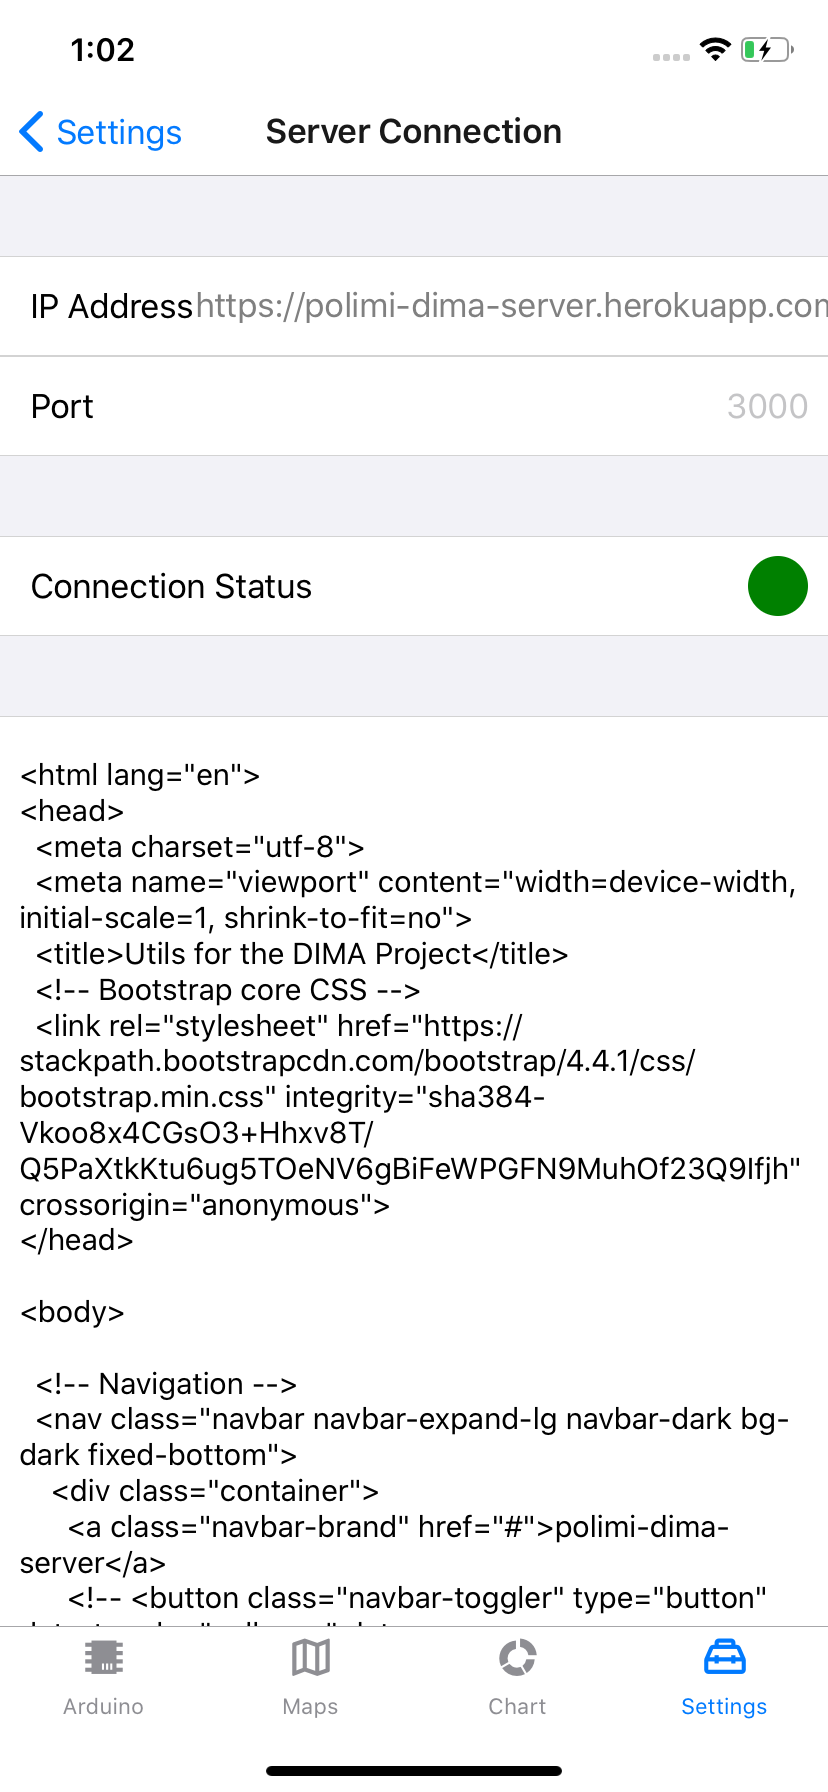
\includegraphics[height=.6\textheight]{./img/ui/server.png}
\caption{\textbf{Connection Screens}}
\end{figure}
\begin{center}
The \textbf{Arduino Connection Screen} and \textbf{Server Connection Screen} allow the user to change the IP address and the port of the \textit{Arduino} board and the \textit{Application Server}.
\end{center}

\begin{figure}[H]
\centering
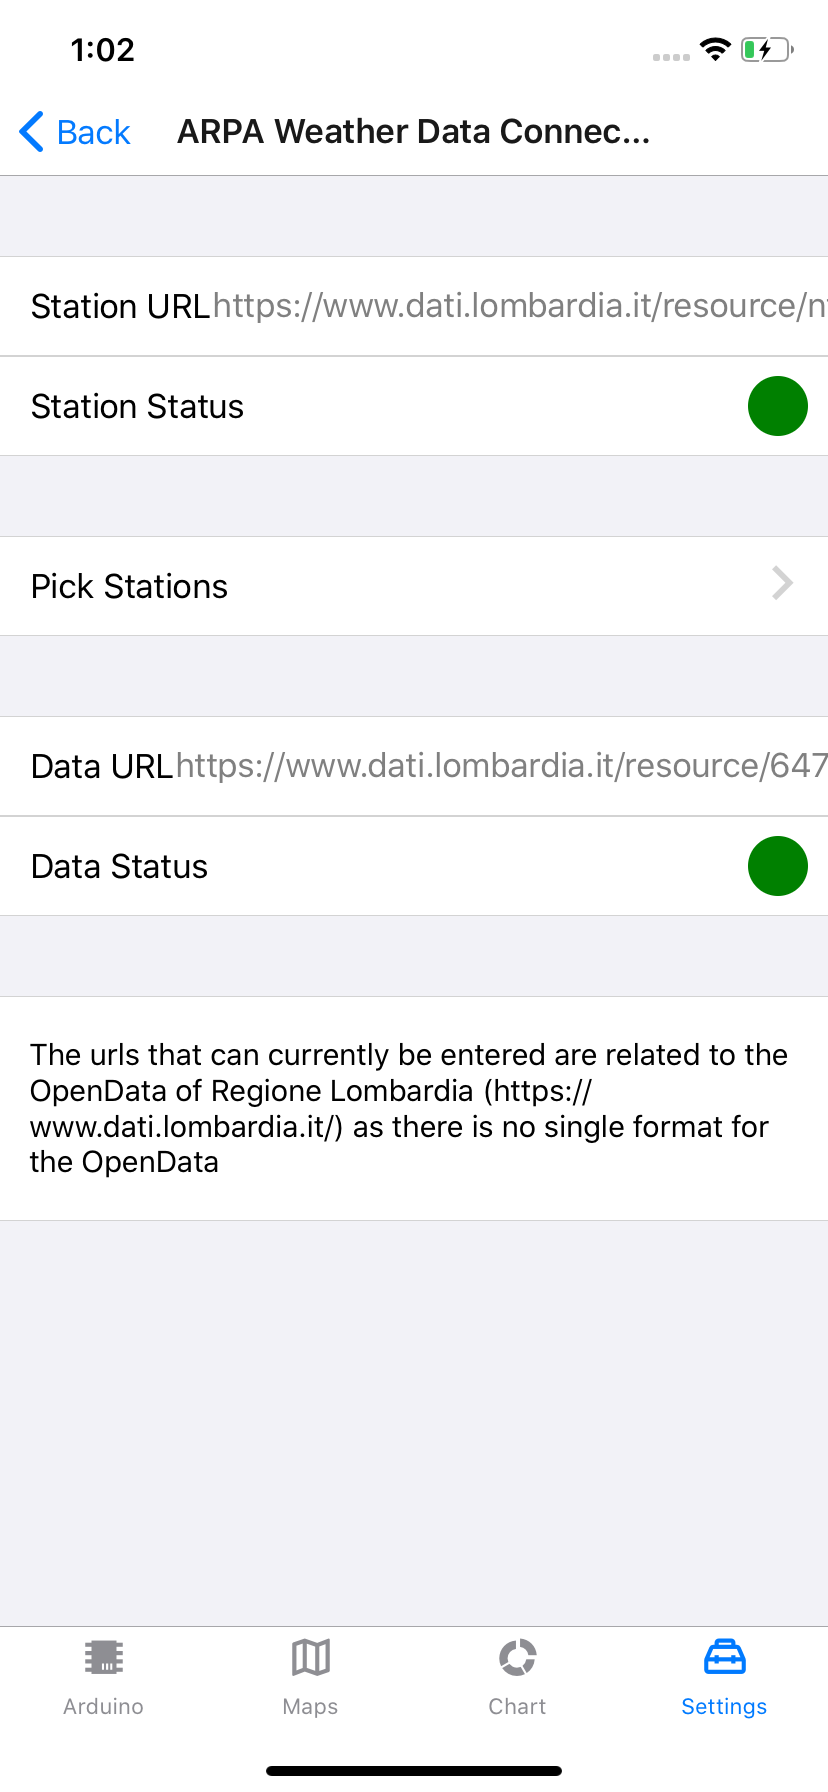
\includegraphics[height=.6\textheight]{./img/ui/arpa_settings.png}
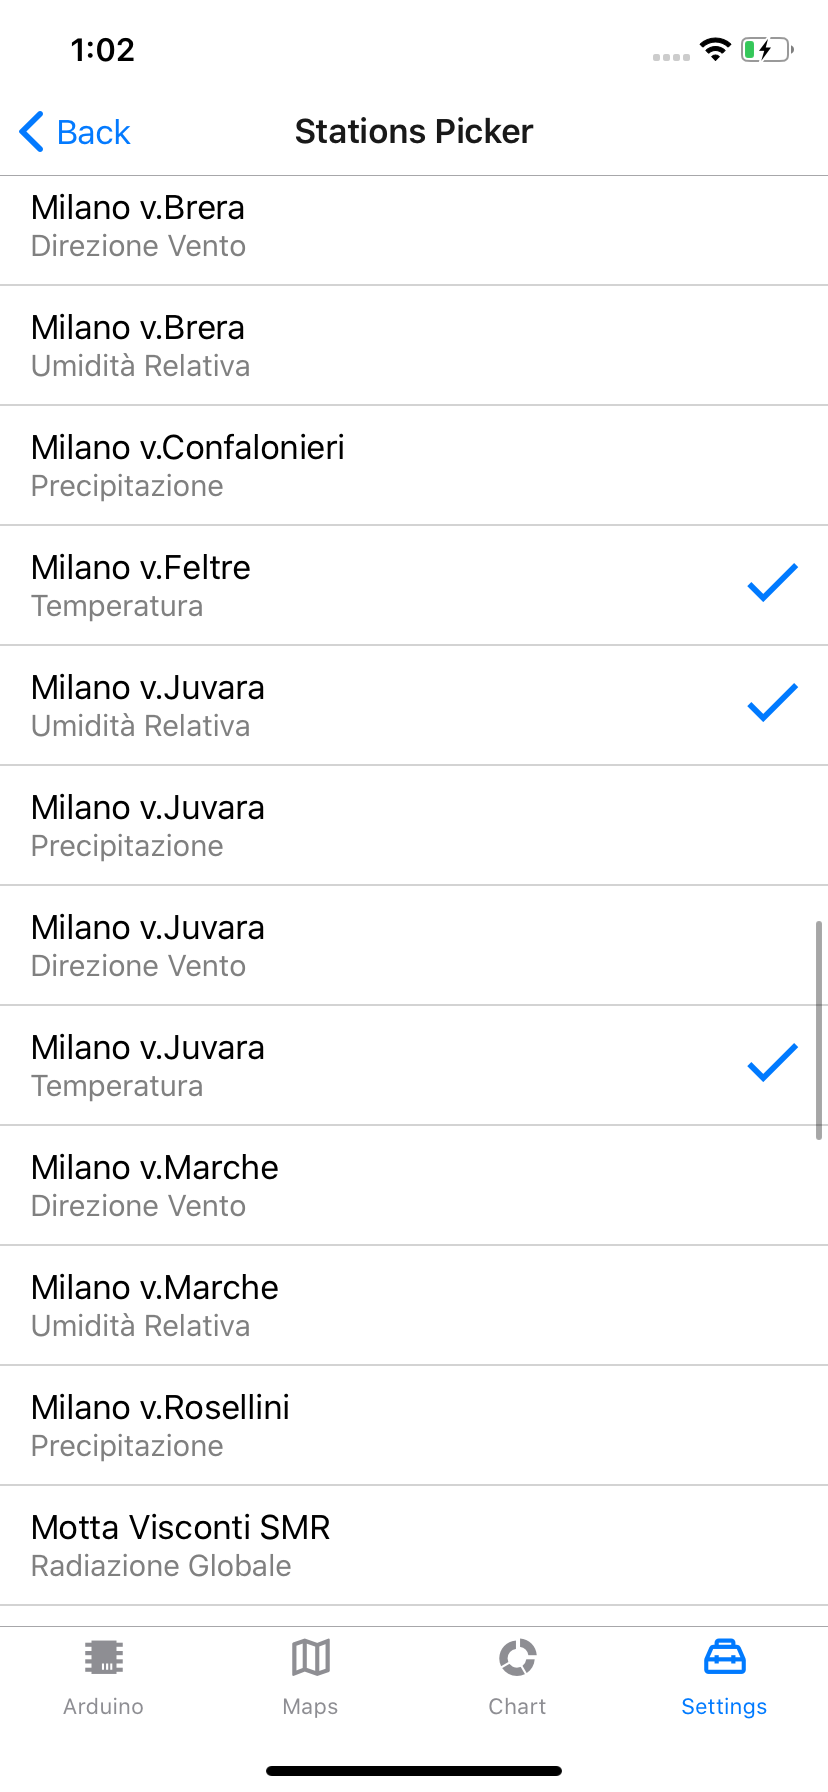
\includegraphics[height=.6\textheight]{./img/ui/stations_picker.png}
\caption{\textbf{ARPA Data Connection Screen}}
\end{figure}
\begin{center}
The \textbf{ARPA Data Connection Screen} allows the user to visualize and change the links of the stations and the data from \textit{Regione Lombardia} OpenData portal.\\ Moreover with the \textbf{Stations Picker Screen} allows the user to select the stations it wants to visualize in the \textbf{Pick Station Screen} of \textbf{Filter Screen}.\\
In the application there are two different \textit{screens}: one for the weather links and an other for the air quality links; however they are managed by the same \textit{Vue Native} component.
\end{center}
\clearpage

% External services and Libraries
\chapter{Frameworks, External services and Libraries}
To develop my application I used \textit{Vue Native} [ \url{https://vue-native.io/} ]; it is a Javascript framework to build cross-platform application that inherits the main features from \textit{Vue.js} and \textit{React Native}.\\ 

\begin{figure}[h]
\begin{center}
  
\includegraphics[width=.5\textwidth]{img/logos/logo_vuenative.png}
  \hspace{0.05\linewidth}
  \centering
  \caption{\textit{Vue Native} logo}
  \label{img:logo_vuenative}
\end{center}
\end{figure}

As in \textit{React Native}, \textit{Vue Native} applications could be built using \textit{Expo} or \textit{React Natice CLI}.\\

\textit{Expo} is designed to allow developers to quickly set up and develop React Native apps, without having to configure Xcode or Android Studio.\\
Since it is most suitable for who come from a Web background, I decided to use it.\\

I also used several external services and libraries.
Some external libraries are necessary for the correct behavior of the application and to have not to waste time in implementing code in order to achieve the objective that these external services already provide.\\

Now, I will present the main external services and libraries that I have used and integreted in \textit{MOQA}.

\section{Vuex}
Vuex is a state management pattern library for \textit{Vue.js} [ \url{https://vuex.vuejs.org/} ] applications. It serves as a centralized store for all the components in an application, with rules ensuring that the state can only be mutated in a predictable fashion. It is based on the state store manager library \textit{Redux} of \textit{React Native}.\\

I have made a custom change to manage the persistence on the phone, using \textit{AsyncStorage} from \textit{React Native} instead of the \textit{localStorage} used in the web.

\medskip
\begin{lstlisting}[style=htmlcssjs]
import {AsyncStorage} from 'react-native';
import store from './index';

const storageKey = '@MySuperStore';

// Function to store the state in the application local storage in the phone
export async function storeData(obj){
  try {
    var copiedObj = JSON.parse(JSON.stringify(obj));
    delete copiedObj.blob;
    // Saving
    await AsyncStorage.setItem(storageKey, JSON.stringify(copiedObj));
    // DEBUG PURPOSE
    await AsyncStorage.getItem(storageKey).then((result) => {console.log("CURRENT AsyncStorage:", result);});
  } catch (error) {
    // Error saving data
  }
}

// Function to get the state saved in the application local storage in the phone
export async function retrieveData(){
  try {
    await AsyncStorage.getItem(storageKey)
    .then((result) => {
      var obj = JSON.parse(result);
      store.commit('REPLACE',obj);
    });
  } catch (error) {
    // Error retrieving data
  }
}

// Function to delete the stored state
export async function deleteDate(){
  try {
    await AsyncStorage.removeItem(storageKey)
    .then((result) => {
      console.log(result);
    });
  } catch (error) {
    // Error retrieving data
  }
}
\end{lstlisting}

\section{Maps, Charts and DateTimePicker}
\textit{Vue Native} has not its own component to build a map or a chart. So, as expleined in the official documentation, I used the community components of \textit{React Native}.\\

It was easy to import the components and the integration does not require any type of effort. Making an example, in the \textit{<script>} section of the code I had to insert:

\medskip
\begin{lstlisting}[style=htmlcssjs]
// Import of MapView from react-native
// react-native-maps is the library maintained
// by the react-native community
import MapView, {Circle} from "react-native-maps";

// Export of the component in Vue Native
export default {
    components: {
      MapView, Circle, Icon
    },
    
}
\end{lstlisting}

Using the above code, in the \textit{<template>} section, we can use \textit{<map-view>} as component of \textit{Vue Native}.

\section{Application Server}
According to the other two people involved in the project, we decided to develop an online RestfulAPI to manage the storage and the retrieve of the data generated by the Arduino board.\\

This RestfulAPI was designed using Swagger [ \url{https://swagger.io/} ], developed using \textit{Node.js} [ \url{https://nodejs.org/} ] framework and delivered with the web-platform \textit{Heroku} [ \url{https://www.heroku.com/} ].\\

\begin{figure}[h]
\begin{center}
  
\includegraphics[width=.5\textwidth]{img/logos/logo_heroku.png}
  \hspace{0.05\linewidth}
  \centering
  \caption{\textit{Heroku} logo}
  \label{img:logo_heroku}
\end{center}
\end{figure}

The web server is available at \url{https://polimi-dima-server.herokuapp.com/}.\\

All the backend is developed using Javascript code and the default \textit{npm} as package manager.\\

The starting point with function declarations and interfaces was generated through the \textit{Swagger} file using the \textit{Swagger Editor} [ \url{https://editor.swagger.io/} ] service.\\

Relevant package added are:
\begin{itemize}
    \item \textit{node-postgres} (aka pg) is a collection of Node.js modules for interfacing with your PostgreSQL database;
    \item \textit{knex.js} is a SQL query builder for Postgres designed to be flexible, portable, and easy to use;
    \item \textit{serve-static} creates a new middleware function to serve files from within a given root directory. The file to serve will be determined by combining req.url with the provided root directory;
    \item \textit{JSON Web Tokens} (aka jwt) is standard method for representing claims securely between two parties. The package allows you to decode, verify and generate JWT .
\end{itemize}

\clearpage
\section{ARPA Data}
ARPA data are not available from the official web-site of the institute, but they are provided by the OpenData service offered by \textit{Regione Lombardia} [ \url{https://www.dati.lombardia.it/} ].\\

\textit{Regione Lombardia} offers a web tool to visualize, aggragate and export data; unlimited downloads of datasets in different formats (e.g. csv, json, ecc...).
Moreover, it offers a web API to access a specific dataset.\\

Data about the monitoring stations are returned as a \textit{GeoJSON} file. The file contains an array of sensors, each one associated to a station, its position, its typology, unit of measure and altitude.\\

Sampled data are returned as objects in an array. For each datum is present the id number of the sensor, the value and the timestamp.

\clearpage

% Test Cases
\chapter{Test Cases}
%input{./files/ux.tex}
\clearpage

% Cost Estimation
\chapter{Effort and Cost Estimation}
%input{./files/ux.tex}
\clearpage

% Future Works
\chapter{Future Works}
In this section I want to analyse the main future works that the project needs.

\begin{itemize}
    \item Since the server is working only as RestfulAPI, as future work it could be considered to implement a web-interface to provide the features now available only with the mobile application.
    \item Now in the \textit{Chart Screen} the visualized data are from a single measure compared with the corresponding available ARPA data from a pinned station; It could be design a system to visualized data coming from different stations or correlate different measures available.
\end{itemize}

\clearpage

\appendix
\chapter{Appendix}
\section{Software and Tools}
\begin{itemize}
  \item \textit{Atom} used as IDE for coding;
  \item \textit{expo.io} used to build, deploy and debug the mobile application;
  \item \textit{Simulator} used to simulate and test the application on an iPhone 11 and an iPad Pro;
  \item \textit{GitHub} used to manage the different versions of the code and this document;
  \item \textit{Swagger} used to design the RestfulAPI of the server;
  \item \textit{Heroku} used to deploy the online server;
  \item \textit{photopea.com} use to draw the application logo and the splash image;
  \item \textit{Balsamiq Mockups 3} used to draw mock-ups;
  \item \text{\LaTeX} used to build this document;
   \item \textit{draw.io} used to draw diagrams.
\end{itemize}


\section{Changelog} \label{Changelog}
\begin{itemize}
  \item \textbf{1.0} : First release of this document.
\end{itemize}
\clearpage

\end{document}